% Set a pdf version and a document type
\ifx\pdfminorversion\undefined\else\pdfminorversion=4\fi
\documentclass[aspectratio=169,t,table]{beamer}

% Import all necessary packages
% Use this file to import all packages which are needed for the lecture
\usepackage[english]{babel}
\usepackage[utf8]{inputenc}
\usepackage[sfdefault]{roboto}
\usepackage[T1]{fontenc}
\usepackage{amsmath,amssymb}
\usepackage{graphicx}
\usepackage{listings}
\usepackage[backend=biber,sorting=none,doi=true,style=ieee]{biblatex}
\usepackage{url}
\usepackage{hyperref}
\usepackage{fontawesome5}
\usepackage{graphicx}
\usepackage{booktabs}
\usepackage{calc}
\usepackage{ifthen}
\usepackage{tabularx}
\usepackage{longtable}
\usepackage{makecell}
\usepackage{multicol}
\usepackage{multirow}
\usepackage{hhline}
\usepackage{qrcode}
\usepackage{xcolor}
\usepackage{cleveref}
\usepackage{tikz}
\usepackage{tikz-cd}
\usepackage{pgfplots,pgfplotstable,pgf-pie}
\usepackage[linesnumbered]{algorithm2e}
\usepackage{array}
\usepackage{mathtools}
\usetikzlibrary{patterns}
\usetikzlibrary{arrows.meta}


% Set the theme (customized FAU beamer theme)
\usetheme[%
	image,%
	longtitle,%
	inst=tf%
]{fau}

% Set all important settings and define commands that are used in more than one lecture
% English version FAU Logo
\usepackage[english]{babel}
% German version FAU Logo
%\usepackage[ngerman]{babel}

\usepackage[utf8]{inputenc}
\usepackage[T1]{fontenc}
\usepackage{amsmath,amssymb}
\usepackage{graphicx}
\usepackage{listings}
\usepackage[backend=biber,sorting=none,doi=true,style=ieee]{biblatex}

% Options:
%  - inst:      Institute
%                 med:      MedFak FAU theme
%                 nat:      NatFak FAU theme
%                 phil:     PhilFak FAU theme
%                 rw:       RWFak FAU theme
%                 rw-jura:  RWFak FB Jura FAU theme
%                 rw-wiso:  RWFak FB WISO FAU theme
%                 tf:       TechFak FAU theme
%  - image:     Cover image on title page
%  - plain:     Plain title page
%  - longtitle: Title page layout for long title
\usetheme[%
	image,%
	longtitle,%
	inst=tf%
]{fau}

% Enable semi-transparent animation preview
\setbeamercovered{transparent}

% Enable frame numbering
%\setbeamertemplate{footline}[frame number]


\lstset{%
	language=Python,
	tabsize=2,
	basicstyle=\tt,
	keywordstyle=\color{blue},
	commentstyle=\color{green!50!black},
	stringstyle=\color{red},
	numbers=left,
	numbersep=0.5em,
	xleftmargin=1em,
	numberstyle=\tt
}

\defbibheading{bibliography}{}
\addbibresource{references.bib}

\date[SS2022]{Summer semester 2022}


\usepackage{url}
\usepackage{enumitem}
\setlist[itemize]{noitemsep, nolistsep}
\setlist[itemize]{label=\footnotesize\raisebox{.275ex}{$\bullet$}}
\usepackage{hyperref}
\usepackage{fontawesome5}
\usepackage{graphicx}
\usepackage{booktabs}
\usepackage{calc}
\usepackage{ifthen}

\usepackage{tabularx}
\usepackage{makecell}

\usepackage{xcolor}
\definecolor{airforceblue}{rgb}{0.36, 0.54, 0.66}
\definecolor{ForestGreen}{rgb}{0.34, 0.139, 0.34}

% English version
\institute[CS6]{Chair of Computer Science 6 (Data Management), Friedrich-Alexander University Erlangen-N\"urnberg}
% German version
% \institute[Lehrstuhl]{Lehrstuhl, Friedrich-Alexander-Universit\"at Erlangen-N\"urnberg}

\setbeamertemplate{section in toc}[sections numbered]

\setbeamertemplate{section page}{%
	\begingroup
	\begin{beamercolorbox}[sep=10pt,center,rounded=true,shadow=true]{section title}
		\usebeamerfont{section title}\thesection~\insertsection\par
	\end{beamercolorbox}
	\endgroup
}

\usepackage{tikz}
\usepackage{tikz-cd}
\usepackage{pgfplots,pgfplotstable,pgf-pie}

\newcommand{\tikzmark}[1]{\tikz[remember picture] \node[coordinate] (#1) {#1};}

\tikzset{
	every overlay node/.style={
			%draw=black,fill=white,rounded corners,
			anchor=north west, inner sep=0pt,
		},
}
% Usage:
% \tikzoverlay at (-1cm,-5cm) {content};
% or
% \tikzoverlay[text width=5cm] at (-1cm,-5cm) {content};
\def\tikzoverlay{%
	\tikz[remember picture, overlay]\node[every overlay node]
}%

\newcommand{\plots}{0.611201}
\newcommand{\plotm}{2.19882}

\newcommand{\MaxNumberX}{3}
\newcommand{\MaxNumberY}{5}

\pgfmathdeclarefunction{gauss}{2}{%
	\pgfmathparse{1/(#2*sqrt(2*pi))*exp(-((x-#1)^2)/(2*#2^2))}%
}

\tikzset{
	thick,
	>=latex,
	every edge/.style={draw=gray, thick, >=latex},
	vertex/.style = {
			circle,
			fill            = black,
			outer sep = 2pt,
			inner sep = 1pt,
		}
}
\usetikzlibrary{matrix,mindmap}
\usetikzlibrary{arrows,decorations.pathmorphing,backgrounds,fit,positioning,shapes.symbols,chains,intersections,snakes}
\tikzset{level 1/.append style={sibling angle=50,level distance = 165mm}}
\tikzset{level 2/.append style={sibling angle=20,level distance = 45mm}}
\tikzset{every node/.append style={scale=1}}
% read in data file
\pgfplotstableread{data/iris.dat}\iris
% get number of data points
\pgfplotstablegetrowsof{\iris}
\pgfmathsetmacro\NumRows{\pgfplotsretval-1}

\usepgfplotslibrary{groupplots}
\pgfplotsset{height=4cm,width=8cm,compat=1.14}

\tikzset{
	vertex/.style = {
			circle,
			fill            = black,
			outer sep = 2pt,
			inner sep = 1pt,
		}
}

\tikzset{
	mynode/.style={
			draw,
			thick,
			anchor=south west,
			minimum width=2cm,
			minimum height=1.3cm,
			align=center,
			inner sep=0.2cm,
			outer sep=0,
			rectangle split,
			rectangle split parts=2,
			rectangle split draw splits=false},
	reverseclip/.style={
			insert path={(current page.north east) --
					(current page.south east) --
					(current page.south west) --
					(current page.north west) --
					(current page.north east)}
		}
}

\tikzset{basic/.style={
			draw,
			rectangle split,
			rectangle split parts=2,
			rectangle split part fill={blue!20,white},
			minimum width=2.5cm,
			text width=2cm,
			align=left,
			font=\itshape
		},
	Diamond/.style={ diamond,
			draw,
			shape aspect=2,
			inner sep = 2pt,
			text centered,
			fill=blue!10!white,
			font=\itshape
		}}


\tikzset{level 1/.append style={sibling angle=50,level distance = 165mm}}
\tikzset{level 2/.append style={sibling angle=20,level distance = 45mm}}
\tikzset{every node/.append style={scale=1}}

\usetikzlibrary{arrows,decorations.pathmorphing,backgrounds,fit,positioning,shapes.symbols,chains,intersections,snakes,positioning,matrix,mindmap,shapes.multipart,shapes,calc,shapes.geometric}



% Title, author(s), and date
\title[KDD~9.~Outlier]{9. Outlier Analysis} %
\subtitle{Knowledge Discovery in Databases}
\author[D.~Probst]{Dominik Probst, \texttt{dominik.probst@fau.de}}

\input{x-additional/vc.tex}

\hypersetup{
	pdfkeywords={},
	pdfsubject={Version \GITAbrHash},
	pdfcreator={},
	pdflang={English}
}


% Create custom commands
\newcommand*\eqmark[3]{{\color{#1}\underbrace{\color{black}#2}_{\tikzmark{#3}}}}

% Set custom (theme) settings 
\setbeamercovered{invisible}
\DeclarePairedDelimiter{\ceil}{\lceil}{\rceil}

% Start the document
\begin{document}

% Title
\maketitle

{ % Outline
	\setbeamertemplate{footline}{}
	\begin{frame}[noframenumbering]{Outline}
		\tableofcontents

	\end{frame}
}

% Body
\section{Outlier and Outlier Analysis}


\begin{frame}{What are Outliers?}
	\begin{block}{Outlier}
		An \textit{outlier} is a data tuple that \underline{deviates significantly} from normal data tuples as if generated by a different mechanism.
	\end{block}

	\begin{itemize}
		\item \textbf{Outliers are \textcolor{faugray}{different from noise}.}
		      \begin{itemize}
			      \item Noise is a random error or variance in a measured variable.
			      \item Noise should be removed before outlier detection.
		      \end{itemize}
		\item \textbf{Outliers are \textcolor{faugray}{interesting}.}
		      \begin{itemize}
			      \item They violate the mechanism that generates data tuples that are considered normal.
			      \item Could occur by chance, measurement error, or any other reason.\newline $\rightarrow$ Justification \textit{why} a tuple is an outlier is important.
		      \end{itemize}
		\item \textbf{Outlier detection vs. novelty detection:} Early stage: outlier; but later merged into the model.
		\item \textbf{Applications:} fraud detection, customer segmentation, medical analyis, industry damage detection.
	\end{itemize}

\end{frame}

\begin{frame}{Types of Outliers}
	\tikzoverlay at (11cm,1cm) {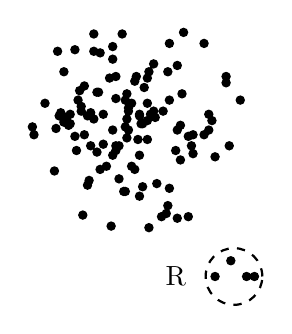
\begin{tikzpicture}[thick,scale=2, every node/.style={scale=5}]
	\fill (1.21, 0.56)  circle (0.3mm) (0.51, 1.02)  circle (0.3mm) (0.61, 1.44)  circle (0.3mm) (0.91, 1.54)  circle (0.3mm) (0.69, 0.58)  circle (0.3mm) (1.2, 1.3)  circle (0.3mm) (1.28, 0.96)  circle (0.3mm) (0.67, 1.21)  circle (0.3mm) (0.34, 0.95)  circle (0.3mm) (0.89, 0.83)  circle (0.3mm) (1.33, 0.38)  circle (0.3mm) (1.3, 1.55)  circle (0.3mm) (1.07, 0.99)  circle (0.3mm) (0.89, 0.62)  circle (0.3mm) (1.07, 0.87)  circle (0.3mm) (0.48, 0.67)  circle (0.3mm) (0.35, 0.9)  circle (0.3mm) (1.26, 1.34)  circle (0.3mm) (0.73, 1.54)  circle (0.3mm) (0.76, 1.17)  circle (0.3mm) (1.02, 1.03)  circle (0.3mm) (1.28, 0.74)  circle (0.3mm) (0.54, 1.3)  circle (0.3mm) (0.73, 1.43)  circle (0.3mm) (0.77, 1.42)  circle (0.3mm) (0.85, 0.93)  circle (0.3mm) (0.97, 1.1)  circle (0.3mm) (1.08, 1.3)  circle (0.3mm) (0.5, 1.43)  circle (0.3mm) (1.25, 0.8)  circle (0.3mm) (1.59, 0.83)  circle (0.3mm) (1.02, 0.51)  circle (0.3mm) (0.79, 0.84)  circle (0.3mm) (1.11, 1.05)  circle (0.3mm) (1.2, 0.45)  circle (0.3mm) (1.66, 1.12)  circle (0.3mm) (0.66, 0.39)  circle (0.3mm) (1.57, 1.27)  circle (0.3mm) (1.19, 0.4)  circle (0.3mm) (0.84, 0.32)  circle (0.3mm) (1.36, 0.9)  circle (0.3mm) (1.21, 1.48)  circle (0.3mm) (1.04, 0.57)  circle (0.3mm) (0.87, 0.83)  circle (0.3mm) (0.92, 0.54)  circle (0.3mm) (0.85, 1.46)  circle (0.3mm) (1.16, 0.38)  circle (0.3mm) (0.94, 0.88)  circle (0.3mm) (1.13, 0.59)  circle (0.3mm) (0.71, 0.83)  circle (0.3mm) (1.26, 0.37)  circle (0.3mm) (1.07, 0.87)  circle (0.3mm) (1.57, 1.23)  circle (0.3mm) (0.62, 0.8)  circle (0.3mm) (1.5, 0.76)  circle (0.3mm) (0.42, 1.1)  circle (0.3mm) (1.43, 1.48)  circle (0.3mm) (1.43, 0.9)  circle (0.3mm) (0.49, 0.94)  circle (0.3mm) (1.08, 0.31)  circle (0.3mm)

	(1.04, 0.97)  circle (0.3mm) (0.95, 0.93)  circle (0.3mm) (1.05, 1.2)  circle (0.3mm) (0.54, 0.98)  circle (0.3mm) (0.71, 1.04)  circle (0.3mm) (0.75, 1.17)  circle (0.3mm) (1.07, 1.26)  circle (0.3mm) (0.63, 1.12)  circle (0.3mm) (0.65, 1.08)  circle (0.3mm) (0.95, 1.05)  circle (0.3mm) (0.83, 1.26)  circle (0.3mm) (0.77, 0.68)  circle (0.3mm) (1.02, 0.77)  circle (0.3mm) (0.64, 1.18)  circle (0.3mm) (0.99, 0.68)  circle (0.3mm) (1.21, 1.12)  circle (0.3mm) (0.75, 0.79)  circle (0.3mm) (1.17, 1.05)  circle (0.3mm) (1.01, 0.87)  circle (0.3mm) (0.69, 1.02)  circle (0.3mm) (1.46, 0.93)  circle (0.3mm) (1.02, 1.02)  circle (0.3mm) (1.26, 0.93)  circle (0.3mm) (1.12, 1.01)  circle (0.3mm) (1.46, 1.03)  circle (0.3mm) (0.93, 0.95)  circle (0.3mm) (0.67, 0.9)  circle (0.3mm) (1.0, 1.27)  circle (0.3mm) (0.99, 1.24)  circle (0.3mm) (0.81, 0.7)  circle (0.3mm) (0.93, 0.54)  circle (0.3mm) (0.97, 0.7)  circle (0.3mm) (0.57, 0.96)  circle (0.3mm) (0.55, 1.01)  circle (0.3mm) (1.33, 0.89)  circle (0.3mm) (0.87, 0.8)  circle (0.3mm) (1.11, 1.35)  circle (0.3mm) (0.85, 1.38)  circle (0.3mm) (0.52, 1.04)  circle (0.3mm) (0.7, 0.61)  circle (0.3mm) (1.48, 0.99)  circle (0.3mm) (1.03, 0.97)  circle (0.3mm) (1.07, 1.1)  circle (0.3mm) (0.65, 1.05)  circle (0.3mm) (0.73, 1.0)  circle (0.3mm) (0.87, 1.13)  circle (0.3mm) (0.87, 1.27)  circle (0.3mm) (1.29, 1.16)  circle (0.3mm) (0.79, 1.03)  circle (0.3mm) (0.94, 1.0)  circle (0.3mm) (0.61, 0.89)  circle (0.3mm) (1.35, 0.83)  circle (0.3mm) (1.36, 0.78)  circle (0.3mm) (0.94, 1.16)  circle (0.3mm) (1.09, 1.03)  circle (0.3mm) (0.85, 0.77)  circle (0.3mm) (0.58, 1.03)  circle (0.3mm) (0.95, 1.07)  circle (0.3mm) (0.58, 0.97)  circle (0.3mm) (0.93, 1.12)  circle (0.3mm);

	\draw[dashed] (1.62,0) circle (1.8mm);
	\fill (1.7,0)  circle (0.3mm) (1.75,0)  circle (0.3mm) (1.5,0)  circle (0.3mm) (1.6,0.1)  circle (0.3mm);
	\node[scale = 0.2] at (1.25,0)    {R};

\end{tikzpicture}
};
	Three kinds: global, contextual, and collective outliers
	\begin{enumerate}
		\item \textbf{Global} outlier (or \textbf{\color{faugray}point anomaly}):
		      \begin{itemize}
			      \item Significantly deviates from the rest of the data set.
			      \item Simplest form of outlier, therefore, most methods focus on finding these.
			      \item Issue: Find an appropriate measurement of deviation.
		      \end{itemize}
		\item \textbf{Contextual} outlier (or \textbf{\color{faugray}conditional outlier}):
		      \begin{itemize}
			      \item Deviates significantly based on a selected context.
			            \begin{itemize}
				            \item Example: Is 23°C in Erlangen an outlier? (Depending on summer or winter).
			            \end{itemize}
			      \item Attributes of data objects divided into two groups:
			            \begin{itemize}
				            \item \textbf{Contextual attributes}: define the context, e.g., time \& location.
				            \item \textbf{Behavioral attributes}: characteristics of the object, used in outlier evaluation, e.g., temperature.
			            \end{itemize}
			      \item Can be viewed as a generalization of local outliers ({\color{faugray} density significantly deviates from its local area}).
			      \item Issue: Formulation of a meaningful context.
		      \end{itemize}
	\end{enumerate}
\end{frame}


\begin{frame}{Types of Outliers (2)}
	\tikzoverlay at (11cm,1cm) {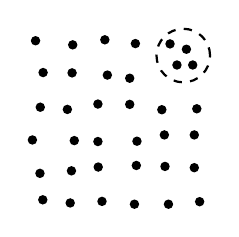
\begin{tikzpicture}[thick,scale=0.4, every node/.style={scale=5}]
	\fill (0.14, 0.02)  circle (1.5mm) (0.05, 0.86)  circle (1.5mm) (-0.19, 1.92)  circle (1.5mm) (0.06, 2.96)  circle (1.5mm) (0.15, 4.06)  circle (1.5mm) (-0.09, 5.07)  circle (1.5mm) (1.01, -0.08)  circle (1.5mm) (1.05, 0.94)  circle (1.5mm) (1.14, 1.9)  circle (1.5mm) (0.92, 2.89)  circle (1.5mm) (1.07, 4.05)  circle (1.5mm) (1.09, 4.94)  circle (1.5mm) (2.02, -0.03)  circle (1.5mm) (1.9, 1.06)  circle (1.5mm) (1.89, 1.87)  circle (1.5mm) (1.89, 3.06)  circle (1.5mm) (2.19, 3.98)  circle 	(1.5mm) (2.11, 5.1)  circle (1.5mm) (3.05, -0.12)  circle (1.5mm) (3.11, 1.11)  circle (1.5mm) (3.13, 1.88)  circle (1.5mm) (2.9, 3.05)  circle (1.5mm) (2.9, 3.88)  circle (1.5mm) (3.08, 4.98)  circle (1.5mm) (4.13, -0.12)  circle (1.5mm) (4.02, 1.08)  circle (1.5mm) (4.0, 2.08)  circle (1.5mm) (3.92, 2.88)  circle (1.5mm) (4.4, 4.3)  circle (1.5mm) (4.18, 4.97)  circle (1.5mm) (5.12, -0.04)  circle (1.5mm) (4.95, 1.04)  circle (1.5mm) (4.95, 2.08)  circle (1.5mm) (5.03, 2.91)  circle (1.5mm) (4.9, 4.3)  circle (1.5mm) (4.7, 4.8)  circle (1.5mm) ;
	\draw[dashed] (4.6,4.6) circle (8.5mm);
\end{tikzpicture}
};
	\begin{enumerate}
		\setcounter{enumi}{2}
		\item \textbf{Collective} outlier:
		      \begin{itemize}
			      \item A \textbf{subset} of data objects that collectively \\
			            deviates significantly from the whole data set.
			      \item Example: intrusion detection -- a number of computers \\
			            keep sending denial-of-service packages to each other.
			      \item \textbf{Detection of collective outliers:}
			            \begin{itemize}
				            \item Consider not only behavior of individual objects, but also that of groups of objects.
				            \item Need to have the background knowledge on the relationship among data objects, such as a distance or similarity measure on objects.
			            \end{itemize}
		      \end{itemize}
	\end{enumerate}

	\begin{alertblock}{Outliers in a Data Set}
		\begin{itemize}
			\item \textbf{A data set may have multiple types of outliers.}
			\item \textbf{One data tuple may belong to more than one type of outlier.}
		\end{itemize}

	\end{alertblock}
\end{frame}


\begin{frame}{Challenges of Outlier Detection}
	\begin{columns}
		\begin{column}{0.55\textwidth}
			\begin{itemize}
				\item \textbf{Modeling normal objects and outliers properly.}
				      \begin{itemize}
					      \item Hard to enumerate all possible normal behaviors in an application.
					      \item No clear line between normal data tuples and outliers.
				      \end{itemize}
				\item \textbf{Application-specific outlier detection.}
				      \begin{itemize}
					      \item Choice of distance measure among objects and the model of \\
					            relationship among objects are application-dependent.
					      \item E.g. clinical data: a small deviation could be an outlier; \\
					            while in marketing analysis: larger fluctuations.
				      \end{itemize}
			\end{itemize}
		\end{column}

		\begin{column}{0.45\textwidth}
			\begin{itemize}
				\item \textbf{Handling noise in outlier detection.}
				      \begin{itemize}
					      \item Noise may distort the normal objects and blur the distinction \\
					            between normal objects and outliers.
					      \item It may hide outliers and reduce the effectiveness of outlier detection.
				      \end{itemize}
				\item \textbf{Understandability.}
				      \begin{itemize}
					      \item Understand why these are outliers: justification of the detection.
					      \item Specify the degree of an outlier: \\
					            the unlikelihood of the object being generated by a normal mechanism.
				      \end{itemize}
			\end{itemize}
		\end{column}
	\end{columns}
\end{frame}

\section{Outlier-Detection Methods}

% TODO: make slide more rounded
\begin{frame}{How can we detect outliers?}
	\textbf{Two ways to categorize outlier-detection methods:}

	Grouping according to
	\begin{enumerate}
		\item \textcolor{faugray}{\textbf{How many samples are labeled:}}\\
		      I.e. supervised, semi-supervised vs. unsupervised methods.
		\item \textcolor{faugray}{\textbf{Assumptions}} regarding normal and abnormal samples.\\
		      I.e. statistical, proximity-based, and clustering-based methods.
	\end{enumerate}
\end{frame}


\begin{frame}{Outlier Detection: Grouping According to Label Existence I}
	Domain expert labelled all, some, or no samples.
	\vspace*{1em}
	\textcolor{faugray}{\textbf{Supervised Methods:}}
	\begin{itemize}
		\item Modeling outlier detection as a \textbf{classification problem}:\\
		      Samples examined by domain experts used for training \& testing.
		\item Methods for learning a classifier for outlier detection effectively:
		      \begin{itemize}
			      \item Model normal objects \& report those not matching the model as outliers.
			      \item Model outliers and treat those not matching the model as normal.
		      \end{itemize}
		\item \textbf{Challenges:}
		      \begin{itemize}
			      \item Imbalanced classes, i.e., outliers are rare: \\
			            Boost the outlier class and make up some artificial outliers.
			      \item Catch as many outliers as possible. \\
			            Therefore: recall is more important than accuracy \\
			            (i.e., not mislabeling normal objects as outliers).
		      \end{itemize}
	\end{itemize}
\end{frame}


\begin{frame}{Outlier Detection: Grouping According to Label Existence II}
	\textcolor{faugray}{\textbf{Unsupervised Methods:}}

	\begin{itemize}
		\item No labels available.
		\item \textbf{Implicit assumptions:}
		      \begin{itemize}
			      \item \textcolor{faugray}{Normal objects are somewhat ``clustered''} into multiple groups, each having some distinct features.
			      \item Outlier are expected to be far away from any group of normal objects.
		      \end{itemize}
		\item Adapt clustering methods for unsupervised outlier detection:
		      \begin{enumerate}
			      \item Find clusters.
			      \item Samples not falling in any cluster are outliers.
		      \end{enumerate}
		\item \textbf{Challenges:}
		      \begin{itemize}
			      \item Samples outside of clusters may not be outliers.
			      \item Costly to find clusters.
			      \item Hard to distinguish noise from outliers.
			      \item Can't detect collective outliers effectively.
		      \end{itemize}
	\end{itemize}
\end{frame}


\begin{frame}
	\frametitle{Outlier Detection: Grouping According to Label Existence III}
	\textcolor{faugray}{\textbf{Semi-Supervised Methods:}}
	\begin{itemize}
		\item Only a small set of samples are labeled as normal or as outlier.
		\item \textbf{If some {\color{airforceblue}labeled normal objects} are available:}
		      \begin{itemize}
			      \item Use the labeled examples and the proximate \\
			            unlabeled objects to train a model for normal objects.
			      \item Those not fitting the model of normal objects are detected as outliers.
		      \end{itemize}
		\item \textbf{If only some {\color{airforceblue}labeled outliers} are available, \\ that small number may not cover all possible outliers well.}
		      \begin{itemize}
			      \item To improve the quality of outlier detection: get help from models for normal objects learned from unsupervised methods.
		      \end{itemize}
	\end{itemize}
\end{frame}


\begin{frame}{Outlier Detection: Grouping Based on Assumption I}
	\tikzoverlay at (11cm,1cm) {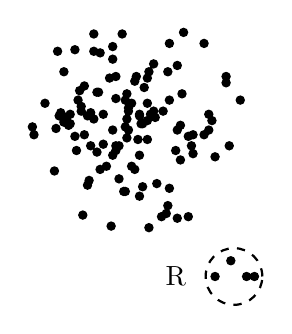
\begin{tikzpicture}[thick,scale=2, every node/.style={scale=5}]
	\fill (1.21, 0.56)  circle (0.3mm) (0.51, 1.02)  circle (0.3mm) (0.61, 1.44)  circle (0.3mm) (0.91, 1.54)  circle (0.3mm) (0.69, 0.58)  circle (0.3mm) (1.2, 1.3)  circle (0.3mm) (1.28, 0.96)  circle (0.3mm) (0.67, 1.21)  circle (0.3mm) (0.34, 0.95)  circle (0.3mm) (0.89, 0.83)  circle (0.3mm) (1.33, 0.38)  circle (0.3mm) (1.3, 1.55)  circle (0.3mm) (1.07, 0.99)  circle (0.3mm) (0.89, 0.62)  circle (0.3mm) (1.07, 0.87)  circle (0.3mm) (0.48, 0.67)  circle (0.3mm) (0.35, 0.9)  circle (0.3mm) (1.26, 1.34)  circle (0.3mm) (0.73, 1.54)  circle (0.3mm) (0.76, 1.17)  circle (0.3mm) (1.02, 1.03)  circle (0.3mm) (1.28, 0.74)  circle (0.3mm) (0.54, 1.3)  circle (0.3mm) (0.73, 1.43)  circle (0.3mm) (0.77, 1.42)  circle (0.3mm) (0.85, 0.93)  circle (0.3mm) (0.97, 1.1)  circle (0.3mm) (1.08, 1.3)  circle (0.3mm) (0.5, 1.43)  circle (0.3mm) (1.25, 0.8)  circle (0.3mm) (1.59, 0.83)  circle (0.3mm) (1.02, 0.51)  circle (0.3mm) (0.79, 0.84)  circle (0.3mm) (1.11, 1.05)  circle (0.3mm) (1.2, 0.45)  circle (0.3mm) (1.66, 1.12)  circle (0.3mm) (0.66, 0.39)  circle (0.3mm) (1.57, 1.27)  circle (0.3mm) (1.19, 0.4)  circle (0.3mm) (0.84, 0.32)  circle (0.3mm) (1.36, 0.9)  circle (0.3mm) (1.21, 1.48)  circle (0.3mm) (1.04, 0.57)  circle (0.3mm) (0.87, 0.83)  circle (0.3mm) (0.92, 0.54)  circle (0.3mm) (0.85, 1.46)  circle (0.3mm) (1.16, 0.38)  circle (0.3mm) (0.94, 0.88)  circle (0.3mm) (1.13, 0.59)  circle (0.3mm) (0.71, 0.83)  circle (0.3mm) (1.26, 0.37)  circle (0.3mm) (1.07, 0.87)  circle (0.3mm) (1.57, 1.23)  circle (0.3mm) (0.62, 0.8)  circle (0.3mm) (1.5, 0.76)  circle (0.3mm) (0.42, 1.1)  circle (0.3mm) (1.43, 1.48)  circle (0.3mm) (1.43, 0.9)  circle (0.3mm) (0.49, 0.94)  circle (0.3mm) (1.08, 0.31)  circle (0.3mm)

	(1.04, 0.97)  circle (0.3mm) (0.95, 0.93)  circle (0.3mm) (1.05, 1.2)  circle (0.3mm) (0.54, 0.98)  circle (0.3mm) (0.71, 1.04)  circle (0.3mm) (0.75, 1.17)  circle (0.3mm) (1.07, 1.26)  circle (0.3mm) (0.63, 1.12)  circle (0.3mm) (0.65, 1.08)  circle (0.3mm) (0.95, 1.05)  circle (0.3mm) (0.83, 1.26)  circle (0.3mm) (0.77, 0.68)  circle (0.3mm) (1.02, 0.77)  circle (0.3mm) (0.64, 1.18)  circle (0.3mm) (0.99, 0.68)  circle (0.3mm) (1.21, 1.12)  circle (0.3mm) (0.75, 0.79)  circle (0.3mm) (1.17, 1.05)  circle (0.3mm) (1.01, 0.87)  circle (0.3mm) (0.69, 1.02)  circle (0.3mm) (1.46, 0.93)  circle (0.3mm) (1.02, 1.02)  circle (0.3mm) (1.26, 0.93)  circle (0.3mm) (1.12, 1.01)  circle (0.3mm) (1.46, 1.03)  circle (0.3mm) (0.93, 0.95)  circle (0.3mm) (0.67, 0.9)  circle (0.3mm) (1.0, 1.27)  circle (0.3mm) (0.99, 1.24)  circle (0.3mm) (0.81, 0.7)  circle (0.3mm) (0.93, 0.54)  circle (0.3mm) (0.97, 0.7)  circle (0.3mm) (0.57, 0.96)  circle (0.3mm) (0.55, 1.01)  circle (0.3mm) (1.33, 0.89)  circle (0.3mm) (0.87, 0.8)  circle (0.3mm) (1.11, 1.35)  circle (0.3mm) (0.85, 1.38)  circle (0.3mm) (0.52, 1.04)  circle (0.3mm) (0.7, 0.61)  circle (0.3mm) (1.48, 0.99)  circle (0.3mm) (1.03, 0.97)  circle (0.3mm) (1.07, 1.1)  circle (0.3mm) (0.65, 1.05)  circle (0.3mm) (0.73, 1.0)  circle (0.3mm) (0.87, 1.13)  circle (0.3mm) (0.87, 1.27)  circle (0.3mm) (1.29, 1.16)  circle (0.3mm) (0.79, 1.03)  circle (0.3mm) (0.94, 1.0)  circle (0.3mm) (0.61, 0.89)  circle (0.3mm) (1.35, 0.83)  circle (0.3mm) (1.36, 0.78)  circle (0.3mm) (0.94, 1.16)  circle (0.3mm) (1.09, 1.03)  circle (0.3mm) (0.85, 0.77)  circle (0.3mm) (0.58, 1.03)  circle (0.3mm) (0.95, 1.07)  circle (0.3mm) (0.58, 0.97)  circle (0.3mm) (0.93, 1.12)  circle (0.3mm);

	\draw[dashed] (1.62,0) circle (1.8mm);
	\fill (1.7,0)  circle (0.3mm) (1.75,0)  circle (0.3mm) (1.5,0)  circle (0.3mm) (1.6,0.1)  circle (0.3mm);
	\node[scale = 0.2] at (1.25,0)    {R};

\end{tikzpicture}
};
	\textcolor{faugray}{\textbf{Statistical Methods}}
	\begin{itemize}
		\item (Also known as model-based methods)
		\item Assume that the \textbf{\color{airforceblue}normal data follow some statistical model}.
		      \begin{itemize}
			      \item The data not following the model are outliers.
		      \end{itemize}
		\item \textbf{Example (right figure):}
		      \begin{itemize}
			      \item First use Gaussian distribution $\mathcal{N}_D(x \; \vert \; \mu,\sigma)$ to model the normal data.
			      \item For each object $y$ in region $R$, estimate $\mathcal{N}_D(y \; \vert \; \mu, \sigma)$, the probability that $y$ \\
			            fits the Gaussian distribution.
			      \item If $\mathcal{N}_D(y \; \vert \; \mu, \sigma)$ is very low, $y$ is unlikely generated by the Gaussian model, thus an outlier.
		      \end{itemize}
		\item\textbf{Effectiveness of statistical methods:}
		      \begin{itemize}
			      \item Highly depends on whether the assumption of statistical model holds in the real data.
		      \end{itemize}
		\item \textbf{There are many kinds of statistical models.}
		      \begin{itemize}
			      \item E.g., parametric vs. non-parametric.
		      \end{itemize}
	\end{itemize}
\end{frame}


\begin{frame}{Outlier Detection: Grouping Based on Assumption II}
	\tikzoverlay at (11cm,1cm) {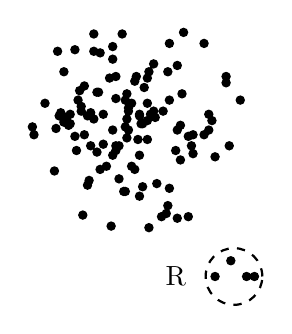
\begin{tikzpicture}[thick,scale=2, every node/.style={scale=5}]
	\fill (1.21, 0.56)  circle (0.3mm) (0.51, 1.02)  circle (0.3mm) (0.61, 1.44)  circle (0.3mm) (0.91, 1.54)  circle (0.3mm) (0.69, 0.58)  circle (0.3mm) (1.2, 1.3)  circle (0.3mm) (1.28, 0.96)  circle (0.3mm) (0.67, 1.21)  circle (0.3mm) (0.34, 0.95)  circle (0.3mm) (0.89, 0.83)  circle (0.3mm) (1.33, 0.38)  circle (0.3mm) (1.3, 1.55)  circle (0.3mm) (1.07, 0.99)  circle (0.3mm) (0.89, 0.62)  circle (0.3mm) (1.07, 0.87)  circle (0.3mm) (0.48, 0.67)  circle (0.3mm) (0.35, 0.9)  circle (0.3mm) (1.26, 1.34)  circle (0.3mm) (0.73, 1.54)  circle (0.3mm) (0.76, 1.17)  circle (0.3mm) (1.02, 1.03)  circle (0.3mm) (1.28, 0.74)  circle (0.3mm) (0.54, 1.3)  circle (0.3mm) (0.73, 1.43)  circle (0.3mm) (0.77, 1.42)  circle (0.3mm) (0.85, 0.93)  circle (0.3mm) (0.97, 1.1)  circle (0.3mm) (1.08, 1.3)  circle (0.3mm) (0.5, 1.43)  circle (0.3mm) (1.25, 0.8)  circle (0.3mm) (1.59, 0.83)  circle (0.3mm) (1.02, 0.51)  circle (0.3mm) (0.79, 0.84)  circle (0.3mm) (1.11, 1.05)  circle (0.3mm) (1.2, 0.45)  circle (0.3mm) (1.66, 1.12)  circle (0.3mm) (0.66, 0.39)  circle (0.3mm) (1.57, 1.27)  circle (0.3mm) (1.19, 0.4)  circle (0.3mm) (0.84, 0.32)  circle (0.3mm) (1.36, 0.9)  circle (0.3mm) (1.21, 1.48)  circle (0.3mm) (1.04, 0.57)  circle (0.3mm) (0.87, 0.83)  circle (0.3mm) (0.92, 0.54)  circle (0.3mm) (0.85, 1.46)  circle (0.3mm) (1.16, 0.38)  circle (0.3mm) (0.94, 0.88)  circle (0.3mm) (1.13, 0.59)  circle (0.3mm) (0.71, 0.83)  circle (0.3mm) (1.26, 0.37)  circle (0.3mm) (1.07, 0.87)  circle (0.3mm) (1.57, 1.23)  circle (0.3mm) (0.62, 0.8)  circle (0.3mm) (1.5, 0.76)  circle (0.3mm) (0.42, 1.1)  circle (0.3mm) (1.43, 1.48)  circle (0.3mm) (1.43, 0.9)  circle (0.3mm) (0.49, 0.94)  circle (0.3mm) (1.08, 0.31)  circle (0.3mm)

	(1.04, 0.97)  circle (0.3mm) (0.95, 0.93)  circle (0.3mm) (1.05, 1.2)  circle (0.3mm) (0.54, 0.98)  circle (0.3mm) (0.71, 1.04)  circle (0.3mm) (0.75, 1.17)  circle (0.3mm) (1.07, 1.26)  circle (0.3mm) (0.63, 1.12)  circle (0.3mm) (0.65, 1.08)  circle (0.3mm) (0.95, 1.05)  circle (0.3mm) (0.83, 1.26)  circle (0.3mm) (0.77, 0.68)  circle (0.3mm) (1.02, 0.77)  circle (0.3mm) (0.64, 1.18)  circle (0.3mm) (0.99, 0.68)  circle (0.3mm) (1.21, 1.12)  circle (0.3mm) (0.75, 0.79)  circle (0.3mm) (1.17, 1.05)  circle (0.3mm) (1.01, 0.87)  circle (0.3mm) (0.69, 1.02)  circle (0.3mm) (1.46, 0.93)  circle (0.3mm) (1.02, 1.02)  circle (0.3mm) (1.26, 0.93)  circle (0.3mm) (1.12, 1.01)  circle (0.3mm) (1.46, 1.03)  circle (0.3mm) (0.93, 0.95)  circle (0.3mm) (0.67, 0.9)  circle (0.3mm) (1.0, 1.27)  circle (0.3mm) (0.99, 1.24)  circle (0.3mm) (0.81, 0.7)  circle (0.3mm) (0.93, 0.54)  circle (0.3mm) (0.97, 0.7)  circle (0.3mm) (0.57, 0.96)  circle (0.3mm) (0.55, 1.01)  circle (0.3mm) (1.33, 0.89)  circle (0.3mm) (0.87, 0.8)  circle (0.3mm) (1.11, 1.35)  circle (0.3mm) (0.85, 1.38)  circle (0.3mm) (0.52, 1.04)  circle (0.3mm) (0.7, 0.61)  circle (0.3mm) (1.48, 0.99)  circle (0.3mm) (1.03, 0.97)  circle (0.3mm) (1.07, 1.1)  circle (0.3mm) (0.65, 1.05)  circle (0.3mm) (0.73, 1.0)  circle (0.3mm) (0.87, 1.13)  circle (0.3mm) (0.87, 1.27)  circle (0.3mm) (1.29, 1.16)  circle (0.3mm) (0.79, 1.03)  circle (0.3mm) (0.94, 1.0)  circle (0.3mm) (0.61, 0.89)  circle (0.3mm) (1.35, 0.83)  circle (0.3mm) (1.36, 0.78)  circle (0.3mm) (0.94, 1.16)  circle (0.3mm) (1.09, 1.03)  circle (0.3mm) (0.85, 0.77)  circle (0.3mm) (0.58, 1.03)  circle (0.3mm) (0.95, 1.07)  circle (0.3mm) (0.58, 0.97)  circle (0.3mm) (0.93, 1.12)  circle (0.3mm);

	\draw[dashed] (1.62,0) circle (1.8mm);
	\fill (1.7,0)  circle (0.3mm) (1.75,0)  circle (0.3mm) (1.5,0)  circle (0.3mm) (1.6,0.1)  circle (0.3mm);
	\node[scale = 0.2] at (1.25,0)    {R};

\end{tikzpicture}
};
	\textcolor{faugray}{\textbf{Proximity-Based Methods}}

	An object is an outlier if the \textbf{\color{airforceblue}nearest neighbors of the object are far away},\\ i.e., the proximity of the object significantly deviates from the proximity\\ of most of the other objects in the same data set.
	\begin{itemize}

		\item \textbf{Example (right figure):}
		      \begin{itemize}
			      \item Model the proximity of an object using its 3 nearest neighbors.
			      \item Objects in region R are substantially different from other objects in the data set.
			      \item Thus the objects in R are outliers.
		      \end{itemize}
		\item \textbf{Effectiveness of proximity-based methods:}
		      \begin{itemize}
			      \item Highly relies on the proximity measure.
			      \item In some applications, proximity or distance measures cannot be obtained easily.
			      \item Often have a difficulty in finding a group of outliers which are close to each other.
		      \end{itemize}
		\item \textbf{Two major types of proximity-based outlier detection:}
		      \begin{itemize}
			      \item Distance-based vs. density-based.
		      \end{itemize}
	\end{itemize}
\end{frame}


\begin{frame}{Outlier Detection: Grouping Based on Assumption III}
	\tikzoverlay at (11cm,1cm) {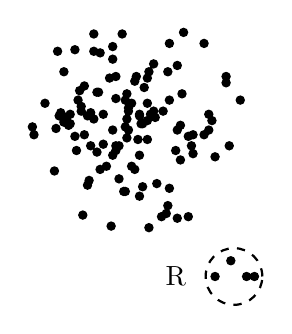
\begin{tikzpicture}[thick,scale=2, every node/.style={scale=5}]
	\fill (1.21, 0.56)  circle (0.3mm) (0.51, 1.02)  circle (0.3mm) (0.61, 1.44)  circle (0.3mm) (0.91, 1.54)  circle (0.3mm) (0.69, 0.58)  circle (0.3mm) (1.2, 1.3)  circle (0.3mm) (1.28, 0.96)  circle (0.3mm) (0.67, 1.21)  circle (0.3mm) (0.34, 0.95)  circle (0.3mm) (0.89, 0.83)  circle (0.3mm) (1.33, 0.38)  circle (0.3mm) (1.3, 1.55)  circle (0.3mm) (1.07, 0.99)  circle (0.3mm) (0.89, 0.62)  circle (0.3mm) (1.07, 0.87)  circle (0.3mm) (0.48, 0.67)  circle (0.3mm) (0.35, 0.9)  circle (0.3mm) (1.26, 1.34)  circle (0.3mm) (0.73, 1.54)  circle (0.3mm) (0.76, 1.17)  circle (0.3mm) (1.02, 1.03)  circle (0.3mm) (1.28, 0.74)  circle (0.3mm) (0.54, 1.3)  circle (0.3mm) (0.73, 1.43)  circle (0.3mm) (0.77, 1.42)  circle (0.3mm) (0.85, 0.93)  circle (0.3mm) (0.97, 1.1)  circle (0.3mm) (1.08, 1.3)  circle (0.3mm) (0.5, 1.43)  circle (0.3mm) (1.25, 0.8)  circle (0.3mm) (1.59, 0.83)  circle (0.3mm) (1.02, 0.51)  circle (0.3mm) (0.79, 0.84)  circle (0.3mm) (1.11, 1.05)  circle (0.3mm) (1.2, 0.45)  circle (0.3mm) (1.66, 1.12)  circle (0.3mm) (0.66, 0.39)  circle (0.3mm) (1.57, 1.27)  circle (0.3mm) (1.19, 0.4)  circle (0.3mm) (0.84, 0.32)  circle (0.3mm) (1.36, 0.9)  circle (0.3mm) (1.21, 1.48)  circle (0.3mm) (1.04, 0.57)  circle (0.3mm) (0.87, 0.83)  circle (0.3mm) (0.92, 0.54)  circle (0.3mm) (0.85, 1.46)  circle (0.3mm) (1.16, 0.38)  circle (0.3mm) (0.94, 0.88)  circle (0.3mm) (1.13, 0.59)  circle (0.3mm) (0.71, 0.83)  circle (0.3mm) (1.26, 0.37)  circle (0.3mm) (1.07, 0.87)  circle (0.3mm) (1.57, 1.23)  circle (0.3mm) (0.62, 0.8)  circle (0.3mm) (1.5, 0.76)  circle (0.3mm) (0.42, 1.1)  circle (0.3mm) (1.43, 1.48)  circle (0.3mm) (1.43, 0.9)  circle (0.3mm) (0.49, 0.94)  circle (0.3mm) (1.08, 0.31)  circle (0.3mm)

	(1.04, 0.97)  circle (0.3mm) (0.95, 0.93)  circle (0.3mm) (1.05, 1.2)  circle (0.3mm) (0.54, 0.98)  circle (0.3mm) (0.71, 1.04)  circle (0.3mm) (0.75, 1.17)  circle (0.3mm) (1.07, 1.26)  circle (0.3mm) (0.63, 1.12)  circle (0.3mm) (0.65, 1.08)  circle (0.3mm) (0.95, 1.05)  circle (0.3mm) (0.83, 1.26)  circle (0.3mm) (0.77, 0.68)  circle (0.3mm) (1.02, 0.77)  circle (0.3mm) (0.64, 1.18)  circle (0.3mm) (0.99, 0.68)  circle (0.3mm) (1.21, 1.12)  circle (0.3mm) (0.75, 0.79)  circle (0.3mm) (1.17, 1.05)  circle (0.3mm) (1.01, 0.87)  circle (0.3mm) (0.69, 1.02)  circle (0.3mm) (1.46, 0.93)  circle (0.3mm) (1.02, 1.02)  circle (0.3mm) (1.26, 0.93)  circle (0.3mm) (1.12, 1.01)  circle (0.3mm) (1.46, 1.03)  circle (0.3mm) (0.93, 0.95)  circle (0.3mm) (0.67, 0.9)  circle (0.3mm) (1.0, 1.27)  circle (0.3mm) (0.99, 1.24)  circle (0.3mm) (0.81, 0.7)  circle (0.3mm) (0.93, 0.54)  circle (0.3mm) (0.97, 0.7)  circle (0.3mm) (0.57, 0.96)  circle (0.3mm) (0.55, 1.01)  circle (0.3mm) (1.33, 0.89)  circle (0.3mm) (0.87, 0.8)  circle (0.3mm) (1.11, 1.35)  circle (0.3mm) (0.85, 1.38)  circle (0.3mm) (0.52, 1.04)  circle (0.3mm) (0.7, 0.61)  circle (0.3mm) (1.48, 0.99)  circle (0.3mm) (1.03, 0.97)  circle (0.3mm) (1.07, 1.1)  circle (0.3mm) (0.65, 1.05)  circle (0.3mm) (0.73, 1.0)  circle (0.3mm) (0.87, 1.13)  circle (0.3mm) (0.87, 1.27)  circle (0.3mm) (1.29, 1.16)  circle (0.3mm) (0.79, 1.03)  circle (0.3mm) (0.94, 1.0)  circle (0.3mm) (0.61, 0.89)  circle (0.3mm) (1.35, 0.83)  circle (0.3mm) (1.36, 0.78)  circle (0.3mm) (0.94, 1.16)  circle (0.3mm) (1.09, 1.03)  circle (0.3mm) (0.85, 0.77)  circle (0.3mm) (0.58, 1.03)  circle (0.3mm) (0.95, 1.07)  circle (0.3mm) (0.58, 0.97)  circle (0.3mm) (0.93, 1.12)  circle (0.3mm);

	\draw[dashed] (1.62,0) circle (1.8mm);
	\fill (1.7,0)  circle (0.3mm) (1.75,0)  circle (0.3mm) (1.5,0)  circle (0.3mm) (1.6,0.1)  circle (0.3mm);
	\node[scale = 0.2] at (1.25,0)    {R};

\end{tikzpicture}
};
	\textcolor{faugray}{\textbf{Clustering-Based Methods}}

	Normal data belong to large and dense clusters, whereas outliers belong to\\ \textbf{\color{airforceblue}small or sparse clusters}, or do not belong to any cluster.
	\begin{itemize}

		\item \textbf{Example (right figure): Two clusters.}
		      \begin{itemize}
			      \item All points not in R form a large cluster.
			      \item The two points in R form a tiny cluster, thus are outliers.

		      \end{itemize}
		\item \textbf{Many clustering methods:}
		      \begin{itemize}
			      \item Thus also many clustering-based outlier detection methods.
		      \end{itemize}
		\item \textbf{Clustering is expensive.}
		      \begin{itemize}
			      \item Straightforward adaptation of a clustering method for outlier detection can be costly and does not scale up well for large data sets.
		      \end{itemize}
	\end{itemize}
\end{frame}

\section{Statistical Approaches}


\begin{frame}{Statistical Approaches}
	\begin{itemize}
		\item \textbf{Assumption:} Objects in a data set are \textbf{\color{airforceblue}generated by a stochastic process} (a generative model).
		\item \textbf{Idea:} Learn a generative model fitting the given data set, and then identify the objects in low-probability regions of the model as outliers.
		\item \textbf{Methods divided into two categories:}
	\end{itemize}
	\vspace*{-2em}
	\begin{columns}
		\begin{column}{0.5\textwidth}
			\begin{center}
				\textbf{Parametric Methods}
			\end{center}
			\vspace*{-1.2em}
			\begin{itemize}
				\item Assumes that the normal data is generated by a parametric distribution with parameter $\theta$.
				\item The probability density function of the parametric distribution $f(x, \theta)$ gives the probability that object $x$ is generated by the distribution.
				\item Small values indicate potential outlier.
			\end{itemize}
		\end{column}
		\begin{column}{0.5\textwidth}
			\pause
			\begin{center}
				\textbf{Non-Parametric Methods}
			\end{center}
			\vspace*{-1.2em}
			\begin{itemize}
				\item Do not assume an a-priori statistical model and determine the model from the input data.
				\item Not completely parameter-free, but consider number and nature of the parameters to be flexible and not fixed in advance.
				\item \textbf{Examples:} \textbf{\color{airforceblue}histogram} and kernel-density estimation.
			\end{itemize}
		\end{column}
	\end{columns}
\end{frame}

\subsection{Parametric Methods}

\begin{frame}{Detection Based on Normal Distribution (I)}
	% TODO: add plot for visual motivation
	\begin{itemize}
		\item \textbf{Univariate data:} A data set involving \textit{only one attribute} or variable.
		\item \textbf{Assumption:} Data are generated from a normal distribution.
		\item \textbf{Learn the parameters from the input data, and identify the points with low probability as outliers.}
	\end{itemize}
	\vspace*{0.5em}
	\textbf{Example:} Assume data follows a \textbf{normal distribution}.
	\begin{itemize}
		\item \underline{Recall:} normal distribution $\mathcal{N}(\mu, \sigma)$
		      \begin{itemize}
			      \item Characterized by two parameters: mean $\mu$, and standard deviation $\sigma$.
			      \item Probability density function: $f(x)=\frac{1}{\sqrt{2\pi \sigma^2}} {\rm e}^{-\frac{(x-\mu)^2}{2\sigma^2}}$.
		      \end{itemize}
		\item \textbf{\color{faugray}Idea:} Estimate parameters $\mu$ and $\sigma$ so that normal distribution fits data as close as possible.
		\item \textbf{Question:} How to estimate these parameters? $\rightarrow$ \textit{\color{faugray}Maximum likelihood method.}
	\end{itemize}
\end{frame}



\begin{frame}{Excursus: Maximum Likelihood Estimation I}
	\begin{block}{Maximum Likelihood Estimation}
		\textit{Maximum Likelihood Estimation} (MLE) estimates \textit{parameters} of an assumed probability distribution such that the \textit{distribution fits the data as closely as possible}.
	\end{block}
	\begin{itemize}
		\item \textbf{Likelihood function} $\mathcal{L}(\theta|X)$ with
		      \begin{itemize}
			      \item parameter space $\theta$ and
			      \item observed data $X=\{x_1, x_2, \dots, x_n\}$
		      \end{itemize}
		      describes the joint probability of observed data as a function of the parameters of the assumed distribution.
		      \begin{itemize}
			      \item Frequently assumed distribution: Gaussian (normal) distribution $\mathcal{N}(\mu, \sigma)$.
			      \item Thus, the likelihood function $\mathcal{L}(\theta|X)$ with parameter space $\theta=\{\mu, \sigma\}$ is the Gaussian process:
			            \begin{equation*}
				            \mathcal{L}(\theta|X)=\mathcal{L}(\mu, \sigma|x_1, \dots, x_n) = \prod\nolimits_{i=1}^n \frac{1}{\sqrt{2\pi \sigma^2}} {\rm e}^{-\frac{(x_i-\mu)^2}{2\sigma^2}}
			            \end{equation*}
		      \end{itemize}
		\item Find good estimates for $\theta$ such that $\widehat{\theta} = \argmax_{\theta} \mathcal{L}(\theta|X)$.
	\end{itemize}
\end{frame}


\begin{frame}{Excursus: Maximum Likelihood Estimation II}
	\begin{itemize}
		\item In the case of a Gaussian distribution: find estimates for $\mu$ and $\sigma$ such that
		      \begin{align*}
			      \widehat{\mu}    & = \textstyle\argmax_{\mu} \mathcal{L}(\theta|X),   \\
			      \widehat{\sigma} & = \textstyle\argmax_{\sigma} \mathcal{L}(\theta|X)
		      \end{align*}
		\item \textbf{General procedure:}
		      \begin{enumerate}
			      \item Generate two derivatives, with respect to $\mu$ and $\sigma$, respectively.
			      \item Solve each equation by setting them equal to zero.
		      \end{enumerate}
		\item Instead of taking the derivative directly, we take the log of the likelihood function as this makes it easier to take derivatives.
		      \begin{equation*}
			      \ln{\mathcal{L}(\theta|x_1, \dots, x_n)}=\ln{\mathcal{L}(\mu, \sigma|x_1, \dots, x_n)}= \ln{\bigg({\textstyle\prod\nolimits_{i=1}^n} \frac{1}{\sqrt{2\pi \sigma^2}} {\rm e}^{-\frac{(x_i-\mu)^2}{2\sigma^2}}\bigg)}
		      \end{equation*}
		      \begin{itemize}
			      \item Logarithm is monotonically increasing, thus satisfying $\argmax_{\theta} \; \ln(\mathcal{L}(\theta|X)) = \text{argmax}_{\theta} \; \mathcal{L}(\theta|X)$.
			      \item Logarithm turns multiplication $\prod$ into addition $\sum$ making derivatives easier to compute.
		      \end{itemize}
	\end{itemize}
\end{frame}
% TODO: MLE easily motivated and explained visually. Maybe insert plots similarly to ML hands-on book p. 269

\begin{frame}{Excursus: Maximum Likelihood Estimation III}
	\begin{enumerate}
		\setcounter{enumi}{-1}
		\item Transform equation:
		      \vspace*{-1em}
		      \begin{equation*}
			      \ln \mathcal{L}(\mu, \sigma | x_1, \dots, x_n) = \ln{\bigg({\textstyle\prod\nolimits_{i=1}^n} \frac{1}{\sqrt{2\pi \sigma^2}} {\rm e}^{-\frac{(x_i-\mu)^2}{2\sigma^2}}\bigg)}= -\frac{n}{2}\ln{2\pi}-\frac{n}{2}\ln{\sigma^2}-\frac{1}{2\sigma^2}\textstyle\sum\nolimits_{i=1}^n (x_i - \mu)^2
		      \end{equation*}
		\item To estimate parameters, take the partial derivative with respect to $\mu$ and $\sigma$:
		      \vspace*{-1em}
		      \begin{align*}
			      \textstyle\frac{\partial}{\partial \mu}\ln{(\mathcal{L}(\mu, \sigma|x_1, \dots, x_n))}    & = \frac{1}{\sigma^2} \sum_{i=1}^n (x_i -\mu)                            \\
			      \textstyle\frac{\partial}{\partial \sigma}\ln{(\mathcal{L}(\mu, \sigma|x_1, \dots, x_n))} & =-\textstyle\frac{n}{\sigma}+\frac{1}{\sigma^3}\sum_{i=1}^n (x_i-\mu)^2
		      \end{align*}
		\item Then, by setting these equations equals zero, we derive the following likelihood estimates:
		      \begin{center}
			      mean $\widehat{\mu}=\frac{1}{n}\sum\nolimits_{i=1}^n x_i$ \hspace{3em} standard deviation $\widehat{\sigma}=\sqrt{\frac{1}{n}\sum\nolimits_{i=1}^n (x_i-\mu)^2}$
		      \end{center}
		      % TODO: proof in appendix or discuss in lecture?
	\end{enumerate}
	\begin{flushright}
		{\color{gray}Refer to appendix for proof.}
	\end{flushright}
\end{frame}

\begin{frame}{Detection Based on Normal Distribution (II)}
	\textbf{Example:}
	\begin{itemize}
		\item Average yearly temperatures: $\{24.0, 28.9, 28.9, 29.0, 29.1, 29.1, 29.2, 29.2, 29.3, 29.4\}$.
		      % TODO: plot data?
		\item For these data with $n = 10$, we have
		      \begin{align*}
			      \widehat{\mu}=28.61, \quad \widehat{\sigma}=\sqrt{2.29}=1.51.
		      \end{align*}
		\item Then the most deviating value $24.0$ is $4.61$ away form the estimated mean.
		\item \textbf{Recall:} $\mu \pm 3\sigma $ contains $99.7\%$ of the data under the assumption of normal distribution.
		\item $\mu \pm 3\sigma$\pause~$ \Leftrightarrow \mu - 3\sigma \leq x \le \mu + 3\sigma$\pause~$ \Leftrightarrow \frac{\mu - x}{\sigma} \leq 3 \leq \frac{\mu + x}{\sigma}$
		\item Plugging in the minimum value ($24.0$) into the equation yields $\frac{\mu-x}{\sigma} = \frac{28.61 - 24}{1.51} =\frac{4.61}{1.51}  =  3.04  >  3$
		\item Probability that $24.0$ is generated by a normal distribution is less than $0.15\%$.
		      \begin{itemize}
			      \item Each \emph{tail} to the left and to the right of the $99.7\%$ has $0.15\%$.
		      \end{itemize}
		\item Hence, $24.0$ identified as an outlier.
	\end{itemize}
\end{frame}


\begin{frame}{The Grubbs' Test\footnote{Named after Frank E. Grubbs.}}
	\begin{block}{Grubbs' Test}
		The \textit{Grubbs' Test} is a statistical test to detect outlier in a \underline{univariate} data set under the assumption that this data set follows a normal distribution. Grubbs' Test is also known as \textit{maximum normed residual test}.
	\end{block}
	\begin{itemize}
		\item Postulates following hypotheses:
		      \begin{itemize}
			      \item $H_0:$ Data set contains no outliers.
			      \item $H_a:$ Data set contains exactly one outlier.
		      \end{itemize}
		\item For a data set $\{x_1, x_2, \dots, x_n\}$ compute the \textbf{Grubbs' test statistic}:  $G = \frac{\max\vert x_i - \overline{x}\vert}{s}$,\\
		      with sample mean $\overline{x}$ and  sample standard deviation $s$.

		\item The two-sided test with significance level $\alpha$ to reject the null hypothesis is as follows:
		      \begin{columns}
			      \begin{column}{0.3\columnwidth}
				      \vspace*{-1em}
				      \begin{flushright}
					      $G > \frac{N-1}{\sqrt{N}} \sqrt{\frac{t^2_{\frac{\alpha}{2N},N-2}}{N-2 + t^2_{\frac{\alpha}{2N},N-2}}}$
				      \end{flushright}
				      \vspace*{0.5em}
			      \end{column}
			      \begin{column}{0.6\columnwidth}
				      where $t^2_{\frac{\alpha}{2N},N-2}$ is the value taken by a $t$-distribution at a significance level of $\frac{\alpha}{2N}$,\\ and $N$ is the number of objects in the data set.
			      \end{column}
		      \end{columns}

	\end{itemize}
\end{frame}


\begin{frame}{Detection of Multivariate Outliers}
	\begin{itemize}
		\item \textbf{Multivariate data}: A data set involving \textbf{\color{faugray}two or more attributes} or variables.
		\item Univariate outlier detection methods can be extended to the multivariate case.
		\item \textbf{Central Idea:} Transform the multivariate outlier-detection task into a univariate outlier-detection problem.
		\item Methods include but not limited to:
		      \begin{enumerate}
			      \item Mahalanobis distance.
			      \item $\chi^2$ statistic
		      \end{enumerate}
	\end{itemize}
	\begin{alertblock}{Beware: Term ``Multivariate'' Defined Differently Throughout Disciplines}
		Depending on the discipline of the paper you may find yourself reading, the term multivariate data, though, maybe misleading. For instance, in probability and statistics, a \textit{multivariate random variable} is a \underline{column vector} $X=\{x_1, x_2, \dots, x_n\}$, i. e. univariate data. However, a \textit{multivariate time series} contains \underline{multiple univariate} time series (column vectors).
	\end{alertblock}
\end{frame}


\begin{frame}{Mahalanobis Distance and $\chi^2$ Statistic}
	\vspace*{-2em}
	\begin{columns}[t]
		\begin{column}{0.5\textwidth}
			\begin{center}
				\textbf{Mahalanobis Distance}
			\end{center}
			\vspace*{-1em}
			\begin{itemize}
				\item Measures the distance between an object $\mathbf{x}$ and the data set's distribution.
				\item Defined as
				      \begin{align*}
					      \text{MD}(\mathbf{x}) = \sqrt{(\mathbf{x} - \mathbf{\overline{x}})^T \mathbf{C}^{-1} (\mathbf{x} - \mathbf{\overline{x}})}
				      \end{align*}
				      with mean $\mathbf{\overline{x}}$, and covariance matrix $\mathbf{C}$, and $\mathbf{x}=(x_1, x_2, \dots, x_n)$ where $x_i$ is a column vector at position $i$.
				\item Use the Grubbs' test on this measure to detect outliers.
			\end{itemize}
		\end{column}

		\begin{column}{0.5\textwidth}
			\begin{center}
				\textbf{$\chi^2$ Statistic}
			\end{center}
			\vspace*{-1em}
			\begin{itemize}
				\item Captures multivariate outliers under the assumption of a normal distribution.
				\item For a data set $\mathbf{x}=(x_1, x_2, \dots, x_n)$, $\chi^2$ statistic is defined as:
				      \begin{align*}
					      \chi^2 = \sum_{i=1}^n \frac{(x_i - \overline{x})^2}{\overline{x}}
				      \end{align*}
				\item If $\chi^2$ statistic is large, then $\mathbf{x}_i$ is an outlier.
			\end{itemize}
		\end{column}
	\end{columns}
\end{frame}

% TODO: Add book author name in footnote
\begin{frame}{Using Mixture of Parametric Distributions}
	\tikzoverlay at (11cm,0.5cm) {\begin{tikzpicture}[
		scale=0.25,
		region./style={
				draw=black,
				shape=circle,
				dashed
			},
		mycircle/.style={
				draw,
				>=latex,
				thick,
				shape=circle,
				fill=black,
				minimum width=0.3em
			},
	]
	\node [mycircle] (1) at (-9.75, -10.25) {};
	\node [mycircle] (3) at (-10.25, -11.5) {};
	\node [mycircle] (4) at (-9.75, -11.75) {};
	\node [mycircle] (5) at (-9, -12.5) {};
	\node [mycircle] (6) at (-8.5, -10.75) {};
	\node [mycircle] (7) at (-10, -10.75) {};
	\node [mycircle] (9) at (-8.5, -11) {};
	\node [mycircle] (10) at (-9, -11) {};
	\node [mycircle] (11) at (-9.25, -11.5) {};
	\node [mycircle] (12) at (-8.75, -11.75) {};
	\node [mycircle] (14) at (-9.5, -10.75) {};
	\node [mycircle] (15) at (-10.25, -10.5) {};
	\node [mycircle] (16) at (-9.75, -11.25) {};
	\node [mycircle] (19) at (-7.75, -11) {};
	\node [mycircle] (20) at (-7.25, -11.75) {};
	\node [mycircle] (21) at (-8.25, -12.5) {};
	\node [mycircle] (22) at (-8.25, -10.25) {};
	\node [mycircle] (25) at (-8, -11.75) {};
	\node [mycircle] (26) at (-8.25, -12) {};
	\node [mycircle] (27) at (-7.5, -11.25) {};
	\node [mycircle] (28) at (-8.75, -9.75) {};
	\node [mycircle] (30) at (-4.5, -11) {};
	\node [mycircle] (31) at (-3, -10) {};
	\node [mycircle] (34) at (-7.5, -10.5) {};
	\node [mycircle] (36) at (-3.5, -9) {};
	\node [mycircle] (37) at (-3.25, -5.25) {};
	\node [mycircle] (38) at (-2.5, -11.75) {};
	\node [mycircle] (39) at (-1.75, -9.25) {};
	\node [mycircle] (41) at (-3, -3) {};
	\node [mycircle] (44) at (-3.75, -5.25) {};
	\node [mycircle] (45) at (-2, -3.75) {};
	\node [mycircle] (47) at (-2.75, -4.25) {};
	\node [mycircle] (53) at (-1.75, -6.75) {};
	\node [mycircle] (56) at (-4.75, -6.25) {};
	\node [mycircle] (57) at (-2.75, -5) {};
	\node [mycircle] (58) at (-4.5, -3.5) {};
	\node [mycircle] (59) at (-3.75, -3) {};
	\node [mycircle] (61) at (-2.5, -3.75) {};
	\node [mycircle] (65) at (-3.25, -4.5) {};
	\node [mycircle] (66) at (-3.75, -3.75) {};
	\node [mycircle] (67) at (-3.25, -4.75) {};
	\node [mycircle] (68) at (-4.25, -4.25) {};
	\node [mycircle] (69) at (-3.75, -4.25) {};
	\node [mycircle] (70) at (-6, -7.25) {};
	\node [mycircle] (71) at (-9.5, -5) {};
	\node [mycircle] (72) at (-4, -4.75) {};
	\node [mycircle] (74) at (-9.25, -4) {};
	\node [mycircle] (78) at (-9.25, -4.75) {};
	\node [mycircle] (79) at (-9.75, -4.5) {};
	\node [mycircle] (80) at (-8.75, -4.25) {};
	\node [mycircle] (81) at (-10.5, -6.5) {};
	\node [mycircle] (82) at (-11.25, -8.25) {};
	\node [mycircle] (83) at (-8.5, -7) {};
	\node [mycircle] (87) at (-2.25, -2.75) {};
	\node [mycircle] (89) at (-9.5, -12.25) {};
	\node [mycircle] (93) at (-7.75, -9.5) {};
	\node [mycircle] (95) at (-3.25, -3.75) {};
	\node [mycircle] (97) at (-2, -4.5) {};
	\node [mycircle] (100) at (-2.25, -3.25) {};
	\node [mycircle] (101) at (-11.25, -3.5) {};
	\node [mycircle] (103) at (-11.5, -2.5) {};
	\node [mycircle] (104) at (-7.25, -3.75) {};
	\node [mycircle] (105) at (-6, -2) {};
	\node [mycircle] (106) at (-9.5, -9.75) {};
	\node [mycircle] (107) at (-9.25, -10.25) {};
	\node (109) at (-1, -4.25) {$C_1$};
	\node (112) at (-8, -4.75) {$C_3$};
	\node (113) at (-6.25, -11.25) {$C_2$};
	\node (114) at (-10.75, -2.75) {$x$};
\end{tikzpicture}
};
	\begin{itemize}
		\item Assuming data follows a normal distribution is too simple for complex\\ data distributions.
		\item Right figure: The objects between the two clusters cannot be captured\\ as outliers since they are close to the estimated mean.
		\item \textbf{Assume data is generated by {\color{airforceblue}two normal distributions.}}
		      \begin{itemize}
			      \item For any object $\mathbf{x}$ in the data set, the probability that $\mathbf{x}$ is generated by the mixture of the two distributions $\mathcal{N}_1(\mu_1, \sigma_1)$ and $\mathcal{N}_2(\mu_2, \sigma_2)$ is given by
			            \begin{align*}
				            \text{P}(\mathbf{x} \; \vert \; \mathcal{N}_1, \mathcal{N}_2) = f_{\mathcal{N}_1}(\mathbf{x} \; \vert \; \mu_1, \sigma_1) + f_{\mathcal{N}_2}(\mathbf{x} \; \vert \; \mu_2, \sigma_2),
			            \end{align*}
			            where $f_{\mathcal{N}_1}$ and $f_{\mathcal{N}_1}$ are the probability density functions of $\mathcal{N}_1$ and $\mathcal{N}_2$, respectively.
			      \item Use expectation-maximization (EM) algorithm\footnote{Expectation-maximization algorithm is not covered in this lecture. If you are interested, you may take a look at chapter 11 of our reference book titled \citetitle{han2011}.} to learn the parameters $\mu_1, \sigma_1, \mu_2, \sigma_2$ from the data.
			      \item An object $\mathbf{x}$ is an outlier if it does not belong to any cluster.
		      \end{itemize}
	\end{itemize}
\end{frame}

\subsection{Non-Parametric Methods}

\begin{frame}{Detection Using Histogram (I)}
	\textit{Non-parametric methods} make fewer assumptions about the data, and thus are applicable in more scenarios.\\\bigskip

	\textbf{Outlier detection using histograms:}
	\begin{columns}
		\begin{column}{0.7\textwidth}
			\vspace*{-1em}
			\begin{enumerate}
				\item Construct histogram
				\item Detect outlier by checking objects against the histogram and determine if is normal or not.\\
				      \textbf{Example:} A transaction with the amount of $\$7,500$ is an outlier, since only $0.2\%$ \\ of the transactions have an amount higher than $\$5,000$.
			\end{enumerate}
		\end{column}
		\begin{column}{0.3\textwidth}
			\begin{figure}
				\centering
				\includegraphics[width=\textwidth]{img/histogram8.png}
			\end{figure}
		\end{column}
	\end{columns}
\end{frame}


\begin{frame}{Detection Using Histogram (II)}
	\textbf{Problem:}
	\begin{itemize}
		\item Hard to \textbf{\color{airforceblue}choose an appropriate bin size} for histogram.
		\item Too small bin size $\rightarrow$ normal objects in empty/rare bins, false positive.
		\item Too big bin size $\rightarrow$ outliers in some frequent bins, false negative.
	\end{itemize}
	\vspace*{1em}
	\textbf{Alternatively:} Estimate probability density function with \textbf{Kernel Density Estimation} (KDE)
	\begin{itemize}
		\item Given: Univariate data set $X=\{x_1, x_2, \dots, x_n\}$ that is drawn i.\,i.\,d (independent and identically distributed)
		\item Its \underline{kernel density estimate} is $\hat{f}_h(x)=\frac{1}{n}\sum_{i=1}^n K_h(x-x_i) = \frac{1}{nh}\sum_{i=1}^n K(\frac{x-x_i}{h})$, where
		      \begin{itemize}
			      \item $\hat{f}$ is the density function to be estimated,
			      \item $h>0$ is a smoothing parameter, also called \textit{bandwidth}, corresponds to the bin width of the histogram. If too small, the curve gets too rough, if too large, shape of $\hat{f}$ is too washed out.
			      \item $K$ is the kernel, a non-negative function, typically standard Gaussian function with $\mu=0$ and $\sigma=1$.
			      \item $K_h$ is the scaled kernel $K_h(x)=\frac{1}{h} K(\frac{x}{h})$
		      \end{itemize}
	\end{itemize}
	% TODO: Add plot of KDE?
\end{frame}

\section{Proximity-Based Approaches}


\begin{frame}{Proximity-Based Approaches}
	\begin{itemize}
		\item \textbf{Assumption:} Outliers are far away
		\item Quantifies how far away objects are from each other by employing a distance measure
		\item Two types of proximity-based outlier detection methods:
	\end{itemize}

	\begin{columns}
		\begin{column}{0.55\textwidth}
			\begin{center}
				\textbf{Distance-Based Methods}
			\end{center}
			\begin{itemize}
				\item Consults the neighborhood.
				\item Neighborhood defined by a given radius.
				\item Objects are considered as outlier if its neighborhood does not contain enough objects.
				\item Different methods: distance-based with nested loop, grid-based.
			\end{itemize}
		\end{column}

		\begin{column}{0.45\textwidth}
			\begin{center}
				\textbf{Density-Based Methods}
			\end{center}
			\begin{itemize}
				\item Investigates the density of an object and that of its neighbors.
				\item Object is considered an outlier if density is lower than that of its neighbors.
			\end{itemize}
		\end{column}
	\end{columns}
\end{frame}

\subsection{Distance-Based Outlier Detection}
\begin{frame}{Method with a Nested Loop (I)}
	\begin{itemize}
		\item Suppose we have:
		      \begin{itemize}
			      \item a set of data objects $D$ with $n$ objects, and
			      \item a user-specified threshold $r$ with $r > 0$
		      \end{itemize}
		\item For each object $\mathbf{o}\in D$ examine the number of other objects in the $r$-neighborhood of $\mathbf{o}$.
		\item If most objects in $D$ are far away from $\mathbf{o}$, then $\mathbf{o}$ is an outlier.
		\item Formally: \textbf{An object $\mathbf{o}$ is a \underline{$\mathbf{DB}(r, \pi)$-outlier}, iff}
		      \begin{align*}\label{db-outlier}
			      \frac{||\{\mathbf{o'} \; \vert \; d(\mathbf{o},\mathbf{o'}) \leq r \}|| }{||D||} \leq \pi.
		      \end{align*}

		      where
		      \begin{itemize}
			      \item $d(\mathbf{o},\mathbf{o}')$ is a distance function of two objects $\mathbf{o}$ and $\mathbf{o}'$
			      \item $\pi$ with $0\leq\pi\leq1$ is a fraction threshold.
		      \end{itemize}
		\item Determine if an object $\mathbf{o}$ is an outlier by taking a look at the $k$-nearest neighbor $\mathbf{o}_k$ where $k=\ceil*{\pi n}$
		\item $\mathbf{o}$ is an outlier, if $d(\mathbf{o}, \mathbf{o}_k) > r$.
	\end{itemize}
\end{frame}

\begin{frame}{Method with a Nested Loop (II)}
	\begin{columns}[t]
		\begin{column}{0.5\textwidth}
			\vspace*{-0.5em}
			\textbf{Efficient computation: {\color{airforceblue}Nested-loop algorithm}:}
			\begin{itemize}
				\item For every object $\mathbf{o}_i\in D$ calculate distance with every other object $\mathbf{o}_j \in D$ where $i\neq j$.
				\item Also count the number of objects in the $r$-neighborhood of $\mathbf{o}_i$.
				\item Terminate inner loop if $\pi n$ objects found in distance $r$: $\mathbf{o}_i$ is no $\mathbf{DB}(r, \pi)$-outlier.
				\item Otherwise do not terminate: $\mathbf{o}_i$ is an outlier.
			\end{itemize}
			\textbf{Efficiency:}
			\begin{itemize}
				\item $\mathcal{O}(n^2)$, but linear CPU-time w.r.t. data set size.
				\item Early termination: small dataset with few outliers.
				\item Costly for large dataset not fitting into RAM.
			\end{itemize}
		\end{column}

		\begin{column}{0.5\textwidth}
			\vspace*{1em}
			\scriptsize
			\begin{algorithm}[H]
				\SetAlgoVlined
				\KwData{a set of objects $D=\{\mathbf{o}_1, \dots, \mathbf{o}_n\}$, threshold $r$, fraction threshold $\pi$}
				\KwResult{$\mathbf{DB}(r, \pi)$-outlier in $D$}
				\BlankLine
				\ForEach{$\mathbf{o}_i\in D$}{
					\texttt{count} $\leftarrow 0$\;
					\ForEach{$\mathbf{o}_j\in D$}{
						\If{$\mathbf{o}_i \neq \mathbf{o}_j$ and $d(\mathbf{o}_i, \mathbf{o}_j)\leq r$}{
							\texttt{count} $\leftarrow$ \texttt{count} $+ 1$\;
							\If{\texttt{count}$\geq \pi n$}{
								\tcc{$\mathbf{o}_i$ cannot be a $\mathbf{DB}(r, \pi)$-outlier}
								exit inner loop\;
							}
						}
					}
				}
				\BlankLine
				\KwRet{
					set of all $\mathbf{DB}(r, \pi)$-outlier in $D$
				}
			\end{algorithm}
		\end{column}
	\end{columns}
\end{frame}


\begin{frame}{Method with a Nested Loop (III)}\textbf{Why is efficiency still a concern?}
	\begin{itemize}
		\item If the complete set of objects cannot be held in main memory, \\
		      there is significant cost for I/O swapping.
	\end{itemize}
	\textbf{The major cost:}
	\begin{enumerate}
		\item \textcolor{faugray}{\textbf{All-Pair-Similarity:}}

		      Each object is tested against the whole data set, \\
		      why not only against its close neighbors?
		\item \textcolor{faugray}{\textbf{Iterative Approach:}}

		      Objects are checked one by one, why not group by group?
	\end{enumerate}

	Improvements can be handled by using a \underline{grid-based method}.
\end{frame}


\begin{frame}{A Grid-Based Method (I)}
	\begin{itemize}
		\item \textbf{CELL:}
		      \begin{itemize}
			      \item Data space is partitioned into a multi-dimensional grid.
			      \item Each cell is a hyper cube with diagonal length $\frac{r}{2}$.
			            \begin{itemize}
				            \item $r$-distance threshold parameter.
				            \item $l$-dimensions: edge of each cell $r / (2\sqrt{l})$ long.
			            \end{itemize}
		      \end{itemize}
		\item \textbf{Level-1 cells:}
		      \begin{itemize}
			      \item Immediately next to cell $\mathbf{C}$.
			      \item For any possible point $\mathbf{x}$ in $\mathbf{C}$ and \\
			            any possible point $\mathbf{y}$ in a level-1 cell: $d(x,y) \leq r$.
		      \end{itemize}
		\item \textbf{Level-2 cells:}
		      \begin{itemize}
			      \item One or two cells away from $\mathbf{C}$.
			      \item For any possible point $\mathbf{x}$ in cell $\mathbf{C}$ and \\
			            any point $\mathbf{y}$ such that $d(x,y) \geq r$, $\mathbf{y}$ is in a level-2 cell.
		      \end{itemize}
		\item Example: Given a 2-dimensional data set, the length of each cell edge is $\frac{r}{2\sqrt{2}}$.
	\end{itemize}
	\tikzoverlay at (10cm,6cm) {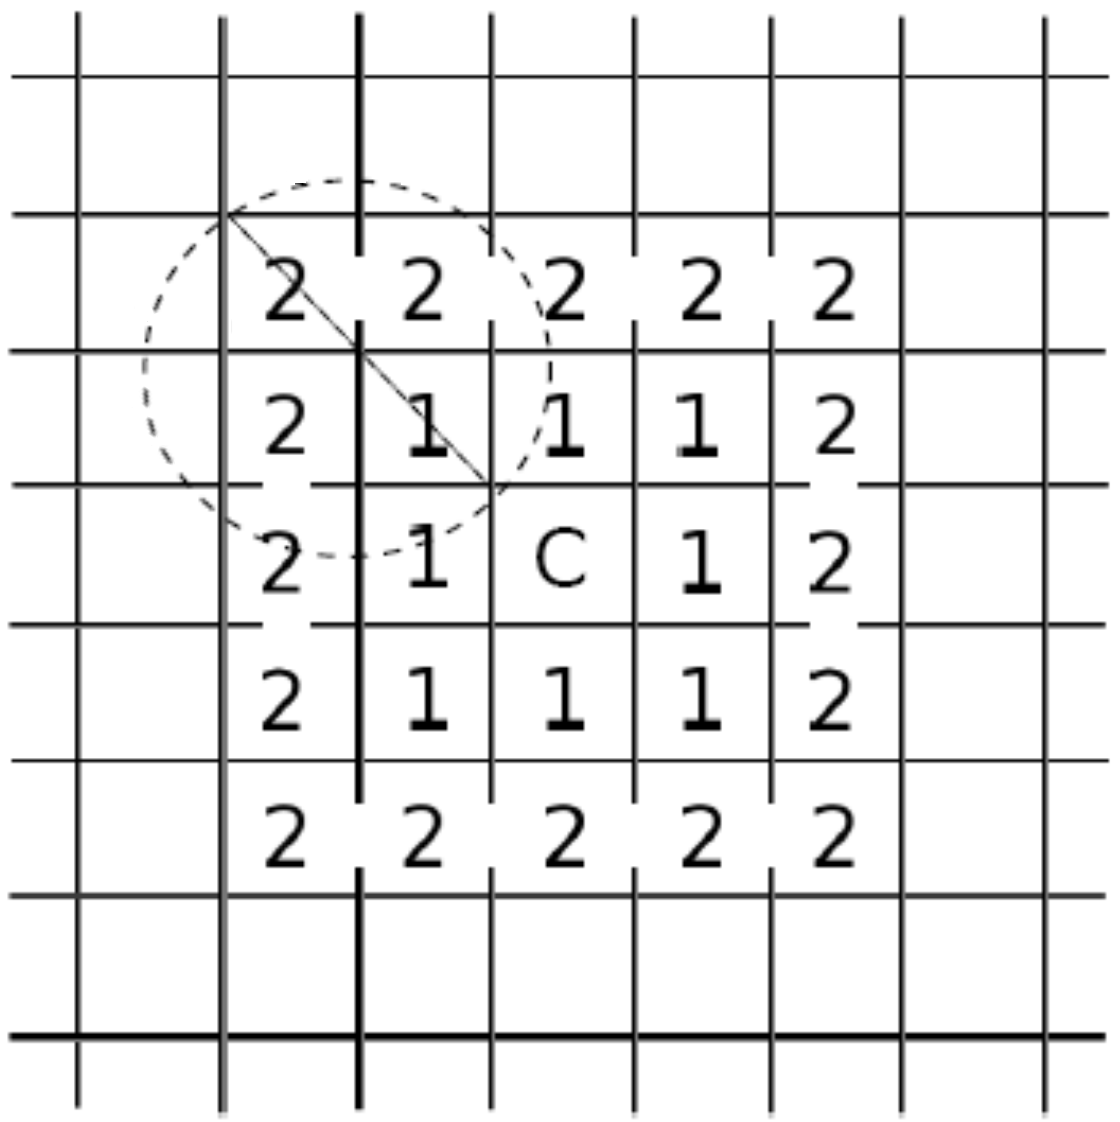
\includegraphics[width=0.25\textwidth]{img/grid8.png}};
\end{frame}


\begin{frame}{A Grid-Based Method (II)}
	\textcolor{faugray}{\textbf{Cell Pruning Rules}}
	\begin{itemize}
		\item Total number of objects in cell $\mathbf{C}$: $a$.
		\item Total number of objects in level-1 cells: $b_1$.
		\item Total number of objects in level-2 cells: $b_2$.
	\end{itemize}
	\begin{itemize}
		\item \textbf{Level-1 cell pruning rule}:
		      \begin{itemize}
			      \item If $a + b_1 > \lceil \pi n \rceil$, then every object $\mathbf{o}$ in $\mathbf{C}$ is not a $\mathbf{DB}(r, \pi)$-outlier, because all objects in $\mathbf{C}$ and the level-1 cells are in the $r$-neighborhood of $\mathbf{o}$, and there are at least $\lceil \pi n \rceil$ such objects.
		      \end{itemize}
		\item \textbf{Level-2 cell pruning rule:}
		      \begin{itemize}
			      \item If $a + b_1 + b_2 < \lceil \pi n \rceil + 1$, then all objects in $\mathbf{C}$ are $\mathbf{DB}(r, \pi)$-outliers, because all of their $r$-neighborhoods have less than $\lceil \pi n \rceil$ other objects.
		      \end{itemize}
		\item \textbf{Only need to check the objects that cannot be pruned.}
		      \begin{itemize}
			      \item Even for such an object $\mathbf{o}$, \\
			            only need to compute the distance between $\mathbf{o}$ and the objects in level-2 cells.
			            \begin{itemize}
				            \item Since beyond level-2, distance from $\mathbf{o}$ is more than $r$.
			            \end{itemize}
		      \end{itemize}
	\end{itemize}
\end{frame}

\subsection{Density-Based Outlier Detection}

\begin{frame}{Density-Based Outlier Detection}
	\begin{itemize}
		\item Density around \textbf{outlier} object \textbf{significantly different}
		\item Methods use a \textit{relative density} of an object against is neighbor.
		\item This indicates to which degree an object is considered an outlier.
		\item \textbf{\color{airforceblue}Local outliers:} Outliers compared to their local neighborhoods, not to global data distribution.
	\end{itemize}
	\vspace*{1em}
	\textbf{Figure on the right:}
	\begin{itemize}
		\item Objects $\textbf{o}_1$ and $\textbf{o}_2$ are local outliers to $C_1$, $\textbf{o}_3$ is a global outlier, \\
		      but $\textbf{o}_4$ is not an outlier.
		\item However, distance of $\textbf{o}_1$ and $\textbf{o}_2$ to objects in dense cluster $C_1$ \\
		      is smaller than average distance in sparse cluster $C_2$.
		\item Hence, $\textbf{o}_1$ and $\textbf{o}_2$ are not distance-based outliers.
	\end{itemize}
	\tikzoverlay at (10cm,3cm) {
		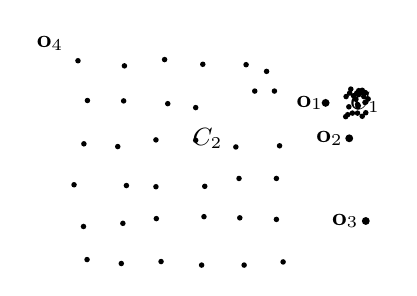
\begin{tikzpicture}[thick,scale=0.5, every node/.style={scale=5}]
			\fill (0.14, 0.02)  circle (0.7mm) (0.05, 0.86)  circle (0.7mm) (-0.19, 1.92)  circle (0.7mm) (0.06, 2.96)  circle (0.7mm) (0.15, 4.06)  circle (0.7mm) (-0.09, 5.07)  circle (0.7mm) (1.01, -0.08)  circle (0.7mm) (1.05, 0.94)  circle (0.7mm) (1.14, 1.9)  circle (0.7mm) (0.92, 2.89)  circle (0.7mm) (1.07, 4.05)  circle (0.7mm) (1.09, 4.94)  circle (0.7mm) (2.02, -0.03)  circle (0.7mm) (1.9, 1.06)  circle (0.7mm) (1.89, 1.87)  circle (0.7mm) (1.89, 3.06)  circle (0.7mm) (2.19, 3.98)  circle (0.7mm) (2.11, 5.1)  circle (0.7mm) (3.05, -0.12)  circle (0.7mm) (3.11, 1.11)  circle (0.7mm) (3.13, 1.88)  circle (0.7mm) (2.9, 3.05)  circle (0.7mm) (2.9, 3.88)  circle (0.7mm) (3.08, 4.98)  circle (0.7mm) (4.13, -0.12)  circle (0.7mm) (4.02, 1.08)  circle (0.7mm) (4.0, 2.08)  circle (0.7mm) (3.92, 2.88)  circle (0.7mm) (4.4, 4.3)  circle (0.7mm) (4.18, 4.97)  circle (0.7mm) (5.12, -0.04)  circle (0.7mm) (4.95, 1.04)  circle (0.7mm) (4.95, 2.08)  circle (0.7mm) (5.03, 2.91)  circle (0.7mm) (4.9, 4.3)  circle (0.7mm) (4.7, 4.8)  circle (0.7mm);

			% cluster
			\fill (7.22, 4.02)  circle (0.7mm) (7.01, 3.74)  circle (0.7mm) (7.17, 4.16)  circle (0.7mm) (7.04, 4.31)  circle (0.7mm) (7.28, 4.1)  circle (0.7mm) (7.22, 3.75)  circle (0.7mm) (6.99, 4.25)  circle (0.7mm) (7.13, 3.66)  circle (0.7mm) (7.03, 3.93)  circle (0.7mm) (6.84, 4.35)  circle (0.7mm) (6.72, 4.16)  circle (0.7mm) (7.14, 4.27)  circle (0.7mm) (6.88, 3.74)  circle (0.7mm) (7.04, 4.21)  circle (0.7mm) (6.79, 3.9)  circle (0.7mm) (7.01, 3.96)  circle (0.7mm) (7.13, 4.32)  circle (0.7mm) (6.71, 3.65)  circle (0.7mm) (6.76, 3.7)  circle (0.7mm) (7.21, 4.26)  circle (0.7mm) (7.02, 3.9)  circle (0.7mm) (7.2, 4.01)  circle (0.7mm) (6.91, 4.18)  circle (0.7mm) (6.81, 4.25)  circle (0.7mm) (6.97, 4.09)  circle (0.7mm);

			% outlier O3
			\fill (7.22, 1)  circle (1mm);
			\node[scale = 0.2] at (6.7, 1) {\small $\textbf{o}_3$};

			% O1
			\fill (6.2, 4)  circle (1mm);
			\node[scale = 0.2] at (5.8, 4) {\small $\textbf{o}_1$};

			% O2
			\fill (6.8, 3.1)  circle (1mm);
			\node[scale = 0.2] at (6.3, 3.1) {\small $\textbf{o}_2$};
			\node[scale = 0.2] at (7.2, 4) {\small $C_1$};
			\node[scale = 0.2] at (3.2, 3.1) {\small $C_2$};
			\node[scale = 0.2] at (-0.8, 5.5) {\small $\textbf{o}_4$};
		\end{tikzpicture}};
\end{frame}


\begin{frame}{Measure Relative Density}
	\begin{itemize}
		\item Use the \textbf{relative density} of an object against its neighbors \\
		      as the indicator of the degree of the object being an outlier.
		\item \textbf{{\color{airforceblue}$k$-distance} of an object $\mathbf{o}$:} $d_k(\mathbf{o})$.

		      Distance between $\mathbf{o}$ and its $k$-nearest neighbors.
		\item Distance $d(\mathbf{o}, \mathbf{p})$ between $\mathbf{o}$ and its $k$-nearest neighbor $p$.
		      \begin{itemize}
			      \item At least $k$-objects $\textbf{o}' \in \mathbf{D} - \{\mathbf{o}\}$
			            such that $d(\mathbf{o}, \mathbf{o}') \leq d(\mathbf{o}, \mathbf{p})$.
			      \item At most $k-1$ objects $\mathbf{o}'' \in \mathbf{D} - \{\mathbf{o}\}$
			            such that $d(\mathbf{o}, \mathbf{o}'') > d(\mathbf{o}, \mathbf{p})$.
		      \end{itemize}
		\item $k$-distance neighborhood of $\mathbf{o}$:
		      \begin{itemize}
			      \item $N_k(\mathbf{o}) = \{\mathbf{o}' \; \vert \; \mathbf{o}' \in \mathbf{D}, d(\mathbf{o}, \mathbf{o}') \leq d_k(\mathbf{o})\}$.
			      \item $N_k(\mathbf{o})$ could be bigger than $k$ \\
			            since multiple objects may have identical distance to $\mathbf{o}$.
		      \end{itemize}
		\item Measure local distance by using the \textit{average distance} from objects in $N_k(\mathbf{o})$.
		\item \textbf{Problem:} If $\mathbf{o}$ has very close neighbors $\mathbf{o}'$, statistical fluctuations of the distance measure can be undesirable high. Overcome this problem with a \underline{reachability distance}.
	\end{itemize}
\end{frame}


\begin{frame}{Reachability Distance}
	\begin{itemize}
		\item \textbf{\color{airforceblue}Reachability distance from $\mathbf{o'}$ to $\mathbf{o}$:}
		      \begin{align*}
			      \text{reachdist}_k(\mathbf{o}' \leftarrow \mathbf{o}) = \max \{d_k(\mathbf{o}), d(\mathbf{o},\mathbf{o}')\},
		      \end{align*}

		      where $k$ is a user-specified parameter that adds a smoothing effect.
		\item $k$ specifies the minimum neighborhood to be examined to determine the local density of an object.
		\item \textbf{Reachability distance is not symmetric!}
		      \begin{align*}
			      \text{reachdist}_k(\mathbf{o}' \leftarrow \mathbf{o}) \neq \text{reachdist}_k(\mathbf{o} \leftarrow \mathbf{o}')
		      \end{align*}
		\item \textbf{Local reachability density of $\mathbf{o}$:}
		      \begin{align*}
			      \text{lrd}_k(\mathbf{o}) = \frac{||N_k(\mathbf{o})||}{\sum_{\mathbf{o'} \in N_k(\mathbf{o})} \text{reachdist}_k(\mathbf{o'} \leftarrow \mathbf{o})}.
		      \end{align*}
	\end{itemize}
\end{frame}


\begin{frame}{Local Outlier Factor (LOF)}
	\begin{itemize}
		\item LOF is the average of the ratio of the local reachability density of $\mathbf{o}$ and \\
		      those of $\mathbf{o}$'s $k$-nearest neighbors.
		\item The lower $\text{lrd}$ and the higher $\text{lrd}$ of the $k$-nearest neighbors of $\mathbf{o}$,\\
		      then the higher the LOF value.
		\item LOF of $\mathbf{o}$ is defined as:
		      \begin{align*}
			      \text{LOF}_k(\mathbf{o}) = \frac{\sum_{\mathbf{o'} \in N_k(\mathbf{o})} \frac{\text{lrd}_k(\mathbf{o'})}{\text{lrd}_k(\mathbf{o})}}{||N_k(\mathbf{o})||} =
			      \sum_{\mathbf{o'} \in N_k(\mathbf{o})} \text{lrd}_k(\mathbf{o'}) \cdot \sum_{\mathbf{o'} \in N_k(\mathbf{o})} \text{reachdist}_k(\mathbf{o'} \leftarrow \mathbf{o}).
		      \end{align*}
		\item This captures a local outlier whose local density is relatively low comparing to the local densities of its $k$-NN.

	\end{itemize}

\end{frame}

\section{Summary}

\begin{frame}
	\frametitle{Summary}
	\begin{itemize}
		\item  \textbf{Types of outliers:}
		      \begin{itemize}
			      \item Global, contextual \& collective outliers.
		      \end{itemize}
		\item \textbf{Outlier detection:}
		      \begin{itemize}
			      \item Supervised, semi-supervised, or unsupervised.
		      \end{itemize}
		\item \textbf{Statistical (or model-based) approaches.}
		\item \textbf{Proximity-based approaches.}
		\item \textbf{Not covered here:}
		      \begin{itemize}
			      \item Clustering-based approaches.
			      \item Classification approaches.
			      \item Mining contextual and collective outliers.
			      \item Outlier detection in high dimensional data.
		      \end{itemize}
	\end{itemize}
\end{frame}

\begin{frame}[c]
	\begin{center}
		{\bf Any questions about this chapter?}\\[0.5cm]
		Ask them now or ask them later in our forum: \\\bigskip
		\qrcode{https://www.studon.fau.de/studon/goto.php?target=lcode_OLYeD79h} \\
		\vspace*{0.5cm}
		\faLink\ \url{https://www.studon.fau.de/studon/goto.php?target=lcode_OLYeD79h} \smallskip

	\end{center}
\end{frame}

\appendix
\section{Appendix}

\begin{frame}{Maximum Likelihood Estimation (MLE)}
	\begin{itemize}
		\item \textbf{Example:} Assume a normal distribution $\mathcal{N}(\mu, \sigma)$ with probability density function
		      \begin{align*}
			      f(x)=\frac{1}{\sqrt{2\pi \sigma^2}} {\rm e}^{-\frac{(x-\mu)^2}{2\sigma^2}}
		      \end{align*}
		\item Likelihood function of the normal distribution for a dataset $X=\{x_1, \dots, x_n\}$, therefore, is as follows:
		      \vspace{-0.8em}
		      \begin{equation*}
			      \mathcal{L}(\mu, \sigma|x_1, \dots, x_n) = \prod\nolimits_{i=1}^n \frac{1}{\sqrt{2\pi \sigma^2}} {\rm e}^{-\frac{(x_i-\mu)^2}{2\sigma^2}}
		      \end{equation*}
		\item General procedure:
		      \begin{enumerate}
			      \item Generate two derivatives, with respect to $\mu$ and $\sigma$, respectively.
			      \item Solve each equation by setting them equal to zero.
		      \end{enumerate}
		\item Instead of taking the derivative directly, we take the log of the likelihood function as this makes it easier to take derivatives.
	\end{itemize}
\end{frame}

\begin{frame}{MLE: Log-Transform Equation}
	\begin{columns}
		\begin{column}{0.6\textwidth}
			\vspace*{-2em}
			\begin{align*}
				 & \ln{\mathcal{L}(\mu, \sigma|x_1, \dots, x_n)}= \ln{\bigg(\eqmark{faured}{\textstyle\prod\nolimits_{i=1}^n}{e1} \frac{1}{\sqrt{2\pi \sigma^2}} {\rm e}^{-\frac{(x_i-\mu)^2}{2\sigma^2}}\bigg)}      \\
				 & =\textstyle\sum\nolimits_{i=1}^n \ln{\bigg(\eqmark{faured}{\frac{1}{\sqrt{2\pi \sigma^2}} {\rm e}^{-\frac{(x_i-\mu)^2}{2\sigma^2}}}{e2}\bigg)}                                                     \\
				 & =\textstyle\sum\nolimits_{i=1}^n \bigg(\ln{\bigg(\eqmark{faured}{\frac{1}{\sqrt{2\pi \sigma^2}}}{e3}\bigg)} + \ln{\bigg(\eqmark{faured}{{\rm e}^{-\frac{(x_i-\mu)^2}{2\sigma^2}}}{e4}\bigg)}\bigg) \\
				 & =\textstyle\sum\nolimits_{i=1}^n \left(\ln{\left((2\pi\sigma^2)^{-\frac{1}{2}} \right)} - \frac{(x_i-\mu)^2}{2\sigma^2} \ln{{\rm e}}\right)
			\end{align*}

			\begin{tikzpicture}[remember picture,overlay]
				\node[below=-1em of e1] (m1) {\color{faured}\small1.};
				\node[below=-1em of e2] (m2) {\color{faured}\small2.};
				\node[below=-1em of e3] (m2) {\color{faured}\small3.a};
				\node[below=-1em of e4] (m2) {\color{faured}\small3.b};
			\end{tikzpicture}

		\end{column}

		\begin{column}{0.4\textwidth}
			\begin{enumerate}
				{
				\setbeamercolor{enumerate item}{fg=faured}
				\item Log transforms multiplication into addition.
				\item Transform each element in log, that is convert multiplication to addition.
				\item Convert one {\color{faured}(a)} over square root and {\color{faured}(b)} exponent of euler.

				      Recall:
				      \vspace*{-1em}
				      \begin{align*}
					      x^{-v}      & = \frac{1}{x^v}  \\
					      \sqrt[v]{x} & =x^{\frac{1}{v}} \\
					      \ln{x^v}    & =v\ln{x}
				      \end{align*}
				      }
			\end{enumerate}
		\end{column}
	\end{columns}
\end{frame}

\begin{frame}{MLE: Log-Transform Equation}
	\vspace*{-2em}
	\begin{columns}
		\begin{column}{0.5\textwidth}
			\begin{align*}
				 & =\textstyle\sum\nolimits_{i=1}^n \Big(\ln{\Big(\eqmark{faured}{(2\pi\sigma^2)^{-\frac{1}{2}}}{e5} \Big)} - \frac{(x_i-\mu)^2}{2\sigma^2} \eqmark{faured}{\ln{{\rm e}}}{e6}\Big) \\
				 & =\textstyle\sum\nolimits_{i=1}^n \Big(-\frac{1}{2}\ln{\eqmark{faured}{2\pi\sigma^2}{e7}}-\eqmark{faured}{\frac{(x_i-\mu)^2}{2\sigma^2}}{e8}\Big)                                \\
				 & =\textstyle\sum\nolimits_{i=1}^n \Big(-\frac{1}{2}\ln{2\pi}-\frac{1}{2}\eqmark{faured}{\ln{\sigma^2}}{e9}-\frac{(x_i-\mu)^2}{2\sigma^2}\Big)                                    \\
				 & =\textstyle\sum\nolimits_{i=1}^n \Big(-\frac{1}{2}\ln{2\pi}-\eqmark{faured}{\textstyle\frac{1}{2}2}{e10}\ln{\sigma}-\frac{(x_i-\mu)^2}{2\sigma^2}\Big)                          \\
				 & =\textstyle\sum\nolimits_{i=1}^n \left(-\frac{1}{2}\ln{2\pi}-\ln{\sigma}-\frac{(x_i-\mu)^2}{2\sigma^2}\right)\tikzmark{e11}
			\end{align*}
			\begin{tikzpicture}[remember picture,overlay]
				\node[below=-1em of e5] (m1) {\color{faured}\small4.a};
				\node[below=-1em of e6] (m2) {\color{faured}\small4.b};
				\node[below=-1em of e7] (m3) {\color{faured}\small5.a};
				\node[below=-1em of e8] (m4) {\color{faured}\small5.b};
				\node[below=-1em of e9] (m5) {\color{faured}\small6.};
				\node[below=-1em of e10] (m6) {\color{faured}\small7.};
			\end{tikzpicture}
		\end{column}

		\begin{column}{0.5\textwidth}
			\begin{enumerate}
				{
				\setbeamercolor{enumerate item}{fg=faured}
				\setcounter{enumi}{3}
				\item Convert {\color{faured}(a)} exponent into multiplication and {\color{faured}(b)} remove $\ln{\rm e}$.

				      Recall:
				      \vspace*{-1em}
				      \begin{align*}
					      \ln{\rm e}=1
				      \end{align*}
				\item {\color{faured}(a)} Transform multiplication to addition. {\color{faured}(b)} Nothing to do to last term.
				\item Convert exponent.
				\item Simplify equation.
				      }
			\end{enumerate}

			\vspace*{1em}
			\textbf{We can now take the derivative w.\,r.\,t. $\mu$ and $\sigma$ of:}
			\vspace*{-1em}
			\begin{align*}
				 & \ln{(\mathcal{L}(\mu, \sigma|x_1, \dots, x_n))}                                                        \\
				 & \tikzmark{e12}=-\textstyle\frac{n}{2}\ln{2\pi}-n\ln{\sigma}-\sum_{i=1}^n \frac{(x_i-\mu)^2}{2\sigma^2}
			\end{align*}
			\begin{tikzpicture}[remember picture,overlay]
				\draw[faured,thick,->] ([yshift=1.2mm,xshift=1mm]e11) to[out=5,in=180] ([yshift=1mm,xshift=-1mm]e12) node [above right=0.1em and 3.3em of e11] (m7) {\small{\color{faured}7.}};
			\end{tikzpicture}
		\end{column}
	\end{columns}
\end{frame}

\begin{frame}{MLE: Take Derivative w.\,r.\,t. $\mu$}
	\vspace*{-2em}
	\begin{columns}
		\begin{column}{0.5\textwidth}
			\begin{align*}
				 & \textstyle\frac{\partial}{\partial \mu}\ln{(\mathcal{L}(\mu, \sigma|x_1, \dots, x_n))}                                                                                                                                                                                            \\
				 & =\eqmark{fauorange}{\textstyle\frac{\partial}{\partial \mu}(-\frac{n}{2}\ln{2\pi})}{e1}-\eqmark{fauorange}{\textstyle\frac{\partial}{\partial \mu}(n\ln{\sigma}}{e2})-\sum_{i=1}^{n} \eqmark{fauorange}{\textstyle\frac{\partial}{\partial \mu}\frac{(x_i-\mu)^2}{2\sigma^2}}{e3} \\
				 & =\eqmark{fauorange}{\textstyle\sum_{i=1}^n \frac{-2(x_i-\mu)(-1)}{2\sigma^2}}{e4}                                                                                                                                                                                                 \\
				 & =\textstyle\sum_{i=1}^n\frac{2(x_i-\mu)}{2\sigma^2}                                                                                                                                                                                                                               \\
				 & = \textstyle\sum_{i=1}^n \frac{x_i-\mu}{\sigma^2}                                                                                                                                                                                                                                 \\
				 & = \frac{1}{\sigma^2} \sum_{i=1}^n (x_i -\mu)
			\end{align*}
			\begin{tikzpicture}[remember picture,overlay]
				\node[below=-1em of e1] (m1) {\color{fauorange}\small1.};
				\node[below=-1em of e2] (m2) {\color{fauorange}\small1.};
				\node[below=-1em of e3] (m2) {\color{fauorange}\small2.};
				\node[below=-1em of e4] (m2) {\color{fauorange}\small3.};
			\end{tikzpicture}
		\end{column}
		\begin{column}{0.5\textwidth}
			\begin{enumerate}
				{
				\setbeamercolor{enumerate item}{fg=fauorange}
				\item Derivative of this component can be treated as a constant as it does not contain $\mu$, therefore it equals to zero.
				\item Apply chain rule.
				\item Simplify equation.
				      }
			\end{enumerate}
			\vspace*{1em}
			{
				\footnotesize
				Recall:
				\vspace*{-1em}
				\begin{align*}
					\text{Linearity: } (f+g)'                                        & = f' + g'                                                                       \\
					\text{Product Rule: } (fg)'                                      & = f'g + fg'                                                                     \\
					\text{Quotient: } \left(\textstyle\frac{f}{g}\right)'            & =\textstyle\frac{f'g-fg'}{g^2}                                                  \\
					\text{Chain Rule: } (f(g(x)))'                                   & =f'(g(x))g'(x)                                                                  \\
					\text{also denoted as: } \textstyle\frac{\partial f}{\partial x} & =\textstyle\frac{\partial f}{\partial g}\textstyle\frac{\partial g}{\partial x}
				\end{align*}
			}
		\end{column}
	\end{columns}
\end{frame}

\begin{frame}{MLE: Take Derivative w.\,r.\,t. $\sigma$}
	\begin{columns}
		\begin{column}{0.5\textwidth}
			\vspace*{-2em}
			\begin{align*}
				 & \textstyle\frac{\partial}{\partial \sigma}\ln{(\mathcal{L}(\mu, \sigma|x_1, \dots, x_n))}                                                                                                                                                                                            \\
				 & =\eqmark{faucyan}{\textstyle\frac{\partial}{\partial \sigma}(-\frac{n}{2}\ln{2\pi})}{e1}-\eqmark{faucyan}{\textstyle\frac{\partial}{\partial \sigma}(n\ln{\sigma}}{e2})-\sum_{i=1}^{n} \eqmark{faucyan}{\textstyle\frac{\partial}{\partial \sigma}\frac{(x_i-\mu)^2}{2\sigma^2}}{e3} \\
				 & =-\textstyle\frac{n}{\sigma}\eqmark{faucyan}{-\textstyle\sum_{i-1}^n \frac{(x_i-\mu)^2}{2}(-2)\sigma^{-3}}{e4}                                                                                                                                                                       \\
				% &=-\textstyle\frac{n}{\sigma}+\sum_{i=1}^n \frac{(x_i-\mu)^2}{2}(2)\sigma^{-3}\\
				 & =-\textstyle\frac{n}{\sigma}+\sum_{i=1}^n (x_i-\mu)^2\eqmark{faucyan}{\sigma^{-3}}{e5}                                                                                                                                                                                               \\
				 & =\eqmark{faucyan}{-\textstyle\frac{n}{\sigma}+\sum_{i=1}^n \frac{(x_i-\mu)^2}{\sigma^3}}{e6}                                                                                                                                                                                         \\
				 & =-\textstyle\frac{n}{\sigma}+\frac{1}{\sigma^3}\sum_{i=1}^n (x_i-\mu)^2
			\end{align*}
			\begin{tikzpicture}[remember picture,overlay]
				\node[below=-1em of e1] (m1) {\color{faucyan}\small1.};
				\node[below=-1em of e2] (m2) {\color{faucyan}\small2.};
				\node[below=-1em of e3] (m2) {\color{faucyan}\small3.};
				\node[below=-1em of e4] (m2) {\color{faucyan}\small4.};
				\node[below=-1em of e5] (m2) {\color{faucyan}\small5.};
				\node[below=-1em of e6] (m2) {\color{faucyan}\small6.};
			\end{tikzpicture}
		\end{column}
		\begin{column}{0.5\textwidth}
			\begin{enumerate}
				{
				\setbeamercolor{enumerate item}{fg=faucyan}
				\item Derivative of this component can be treated as a constant as it does not contain $\sigma$, therefore it equals to zero.
				\item Take derivative.
				\item Easier when expressed as $\frac{(x_i-\mu)^2}{2}\sigma^{-2}$. Then take derivative of $\sigma^{-2}$. Recall: $(x^a)'=ax^{a-1}$
				\item Two minuses cancel out (minus before sum and minus of $(-2)$). Additionally, simplify by cancel out $\frac{2}{2}$.
				\item Put back as denominator.
				\item Simplify equation.
				      }
			\end{enumerate}
		\end{column}
	\end{columns}
\end{frame}

\begin{frame}{MLE: Two Derivatives w.\,r.\,t. $\mu$ and $\sigma$}
	\vspace*{-1em}
	Derivatives are:
	\vspace*{-2em}
	\begin{align*}
		\textstyle\frac{\partial}{\partial \mu}\ln{(\mathcal{L}(\mu, \sigma|x_1, \dots, x_n))}    & = \frac{1}{\sigma^2} \sum_{i=1}^n (x_i -\mu)                            \\
		\textstyle\frac{\partial}{\partial \sigma}\ln{(\mathcal{L}(\mu, \sigma|x_1, \dots, x_n))} & =-\textstyle\frac{n}{\sigma}+\frac{1}{\sigma^3}\sum_{i=1}^n (x_i-\mu)^2
	\end{align*}

	\textbf{To find the estimates of $\mu$ and $\sigma$, solve these equations by equal them to zero\footnote{We want to find the value for with the log functions reaches their maximum. At this point, the slope of these functions equal to zero. Therefore, we equal these functions to zero.}:}

	\begin{itemize}
		\item For $\mu$: $0=\textstyle\frac{1}{\sigma^2} \sum_{i=1}^n (x_i -\mu) \stackrel{{\color{faured}\times \sigma^2}}{\Leftrightarrow} 0=\sum_{i=1}^n x_i-\mu \stackrel{{\color{faured}+n\mu}}{\Leftrightarrow} n\mu = \sum_{i=1}^n x_i \stackrel{{\color{faured}\times\frac{1}{n}}}{\Leftrightarrow} \underline{\underline{\mu=\frac{1}{n}\sum_{i=1}^n x_i}}$\\This equals to mean.
		\item For $\sigma$: $0=-\textstyle\frac{n}{\sigma}+\frac{1}{\sigma^3}\sum_{i=1}^n (x_i-\mu)^2 \stackrel{{\color{faured}\times \sigma}}{\Leftrightarrow} 0=-n+\frac{1}{\sigma^2}\sum_{i=1}^n (x_i-\mu)^2 \stackrel{{\color{faured}+n}}{\Leftrightarrow} n=\frac{1}{\sigma^2} \sum_{i=1}^n (x_i-\mu)^2$\\
		      $\stackrel{{\color{faured}\times \sigma^2}}{\Leftrightarrow} n\sigma^2 = \sum_{i=1}^n (x_i-\mu)^2 \stackrel{{\color{faured}\times \frac{1}{n}}}{\Leftrightarrow} \sigma^2 = \frac{1}{n}\sum_{i=1}^n (x_i-\mu)^2 \stackrel{{\color{faured}\sqrt{\vphantom{}}}}{\Leftrightarrow} \underline{\underline{\sigma=\sqrt{\frac{1}{n}\sum_{i=1}^n (x_i-\mu)^2}}}$\\This equals to standard deviation.
	\end{itemize}
\end{frame}

\end{document}
